\documentclass[11pt]{article}

% Packages
\usepackage[T1]{fontenc}
\usepackage[english]{babel}

\usepackage{amsmath, amssymb}

\usepackage{graphicx, caption, subcaption, float, pgfplots, array}
\pgfplotsset{compat=1.18}
\usepackage[a4paper, margin=1in]{geometry}
\geometry{top=2cm, bottom=2cm, left=2.5cm, right=2.5cm}
\usepackage[table]{xcolor}
\usepackage{xcolor}
\usepackage{booktabs}
\usepackage{colortbl}
\usepackage{hhline}
\renewcommand{\arraystretch}{1.5}

\usepackage[colorlinks=true, linkcolor=black, urlcolor=black, citecolor=black]{hyperref}
\hypersetup{colorlinks=true, urlcolor=blue}
\usepackage{fancyhdr}
\setlength{\headheight}{14pt}
\pagestyle{fancy}
\fancyhf{}
\fancyhead[L]{\nouppercase{\leftmark}}
\fancyfoot[C]{\thepage}
\renewcommand{\sectionmark}[1]{\markboth{#1}{}}

% Fancyhdr for headers
\usepackage{fancyhdr}
\setlength{\headheight}{14pt}
\pagestyle{fancy}
\fancyhf{} % Clear default header/footer
\fancyhead[L]{\nouppercase{\leftmark}} % Section in header (left)
\fancyfoot[C]{\thepage} % Page number in footer (center)

\renewcommand{\sectionmark}[1]{\markboth{#1}{}}

\usepackage{url}
\usepackage{breakurl}
\usepackage[backend=biber,style=numeric,url=true]{biblatex}
\addbibresource{../references.bib}
\DeclareFieldFormat{url}{\newline\url{#1}}
\setlength{\bibitemsep}{1em}



% DOCUMENT'S FIRST PAGE ---------------------------------------------------------------------------------------------------------------------
\begin{document}
\thispagestyle{empty}

\begin{flushright}
    
\includegraphics[width=0.4\linewidth]{images/Politecnico di Torino logo}
\end{flushright}

\vspace*{7cm}

\begin{flushleft}
    {\Huge\bfseries Low-cost heavy duty AMR} \\
    \vspace{0.5cm}
    {\Large\bfseries BSc Thesis in Mechanical Engineering} \\
    \vspace{0.5cm}
    {\large A.A. 2024-2025} \\
    \vspace{1cm}

    {\large Candidato: Paradiso Francesco Pio} \\
    \vspace{0.5cm}
    {\large Relatore: Prof. Chiaberge Marcello} \\
\end{flushleft}

\vfill

% ABSTRACT ------------------------------------------------------------------------------------------------------------------------------
\newpage
\thispagestyle{empty}

\section*{Abstract}
This thesis highlights the design, analysis, and manufacture of a low-cost suspension system tailored for a heavy-duty AMR, primarily used for industrial and warehouse applications and environments. Although the thesis focus has been mainly on static scenarios and regular surfaces, the role of a suspension system is pivotal for ensuring traction when it encounters obstacles on the way.

The work begins with a brief review of existing suspension technologies used in robotics and these kind-like applications, spotlighting their limitations in terms of cost and complexity. Building on this, the study outlines the mechanical requirements needed taking into account payload constraints, static and fatigue resistance, considering the DoF available.

Several concepts have been delivered and evaluated through a trade-off analysis combined with cost obligations, leading to the selection of a spring-based passive suspension system since it represents the most viable solution. Furthermore, a detailed CAD model has been developed with parametric design to match spring geometric characteristics.

The performance of the suspension has been validated through both analytical calculations and FEM simulations. Subsequentially, a prototype has been fabricated and tested in controlled conditions to verify real-world performance and identify discrepancies with simulations.

The thesis concludes with a discussion of the strengths and limitations of the design, providing recommendations for further optimization, including potential integration with active damping or adaptive control systems.


% ACKNOWLEDGEMENTS ----------------------------------------------------------------------------------------------------------------------
\newpage
\thispagestyle{empty}

\section*{Acknowledgements}

% TABLE OF CONTENTS ---------------------------------------------------------------------------------------------------------------------
\newpage
\thispagestyle{empty}
\tableofcontents

% LIST OF FIGURES ----------------------------------------------------------------------------------------------------------------------
\newpage
\thispagestyle{empty}
\listoffigures

% LIST OF TABLES -----------------------------------------------------------------------------------------------------------------------
\newpage
\thispagestyle{empty}
\listoftables

% LIST OF ABBREVIATIONS -----------------------------------------------------------------------------------------------------------------
\newpage
\thispagestyle{empty}
\section*{List of Abbreviations}
\begin{itemize}
    \item AMR: Autonomous Mobile Robot
    \item FEM: Finite Element Method
    \item CAD: Computer-Aided Design
\end{itemize}

% SYMBOLS ------------------------------------------------------------------------------------------------------------------------------
\newpage
\thispagestyle{empty}

\section*{List of Symbols}
\begin{tabular}{ll}
    $d$ & Wire diameter [mm] \\
    $D$ & Mean diameter [mm] \\
    $L_0$ & Free length [mm] \\
    $L_\text{Fmax}$ & Maximum force length [mm] \\
    $k$ & Spring constant [N/m] \\
    $\text{CS}_\text{sta}$ & Static safety coefficient \\
    $\text{CS}_\text{fat}$ & Fatigue safety coefficient \\
    $f_\text{ost}$ & Obstacle deflection [mm] \\
    $i_\text{eff}$ & Effective number of turns \\
\end{tabular}

% DOCUMENT'S MAIN CONTENT -------------------------------------------------------------------------------------------------------------------
\newpage
\section{Background and Literature Review}
\subsection{Types of Suspension Systems in Robotics}
Suspension systems in robotics play a central role in maintaining stability, mitigating shocks on uneven terrain, and ensuring consistent ground contact. Accordingly to the mechanical characteristics, they are used for diverse applications:
\begin{itemize}
    \item \textbf{Spring-Damper Suspension} \\ It combines a mechanical spring with a damper for energy absorption and energy dissipation respectively. The system provides a good response to moderate terrain irregularities and its implementation and maintenance simplicity are revealed to be huge benefits.
    \item \textbf{Rocker-Bogie Suspension} \\ Notable for its use in NASA’s Mars rovers, the system enables continuous contact with the ground over highly uneven surfaces. The main advantages are the efficient load distribution and the fact that it does not require active control.
    \item \textbf{Multi-Link Suspension} \\ The arrangement of arms and joints allows precise control over each wheel position and motion, despite its complexity is an engineering challenge. Moreover, it offers enhanced stability and traction, even on high-loading. 
    \item \textbf{Articulated Suspension} \\ It uses rotating joints in the chassis to increase maneuverability and improve terrain adaptability. Usually employed in tracked robots or platforms.
    \item \textbf{Differential Suspension} \\ It allows differential movement between wheels, allowing the robot to adapt to uneven surfaces without particular mechanical complexities.
    \item \textbf{Leaf Spring Suspension} \\ Widely used for larger vehicles, this system uses layered metal strips to support weight-absorbing shocks. In robotics, it is adopted due to its simplicity and high load capacity, despite it offering limited terrain compliance.
\end{itemize}
This variety reflects the trade-offs between complexity, cost, adaptability, and high-load performance in robotic applications which makes the choice of suspension system a critical design decision. 
In the case of this specific application, the suspension system choosen is a spring-damper system, which is the most suitable for the AMR's intended use in industrial and warehouse environments. The design focuses on balancing performance, cost, and ease of maintenance, making it an ideal choice for medium and heavy-duty applications.

\begin{figure}[H]
    \centering
    \subfloat[Spring-Damper \cite{springdamper_source}]{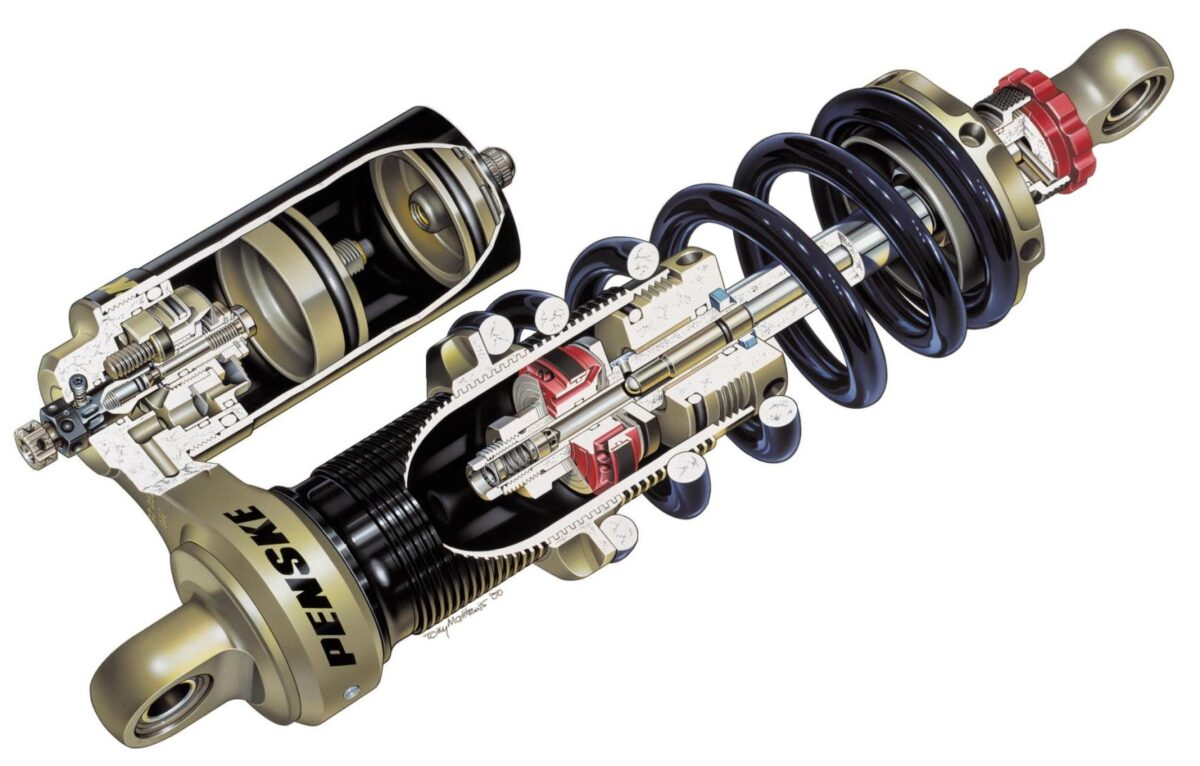
\includegraphics[width=0.21\textwidth]{images/suspensions/Spring-Damper Suspension.jpg}} \quad
    \subfloat[Rocker-Bogie \cite{rockerbogie_source}]{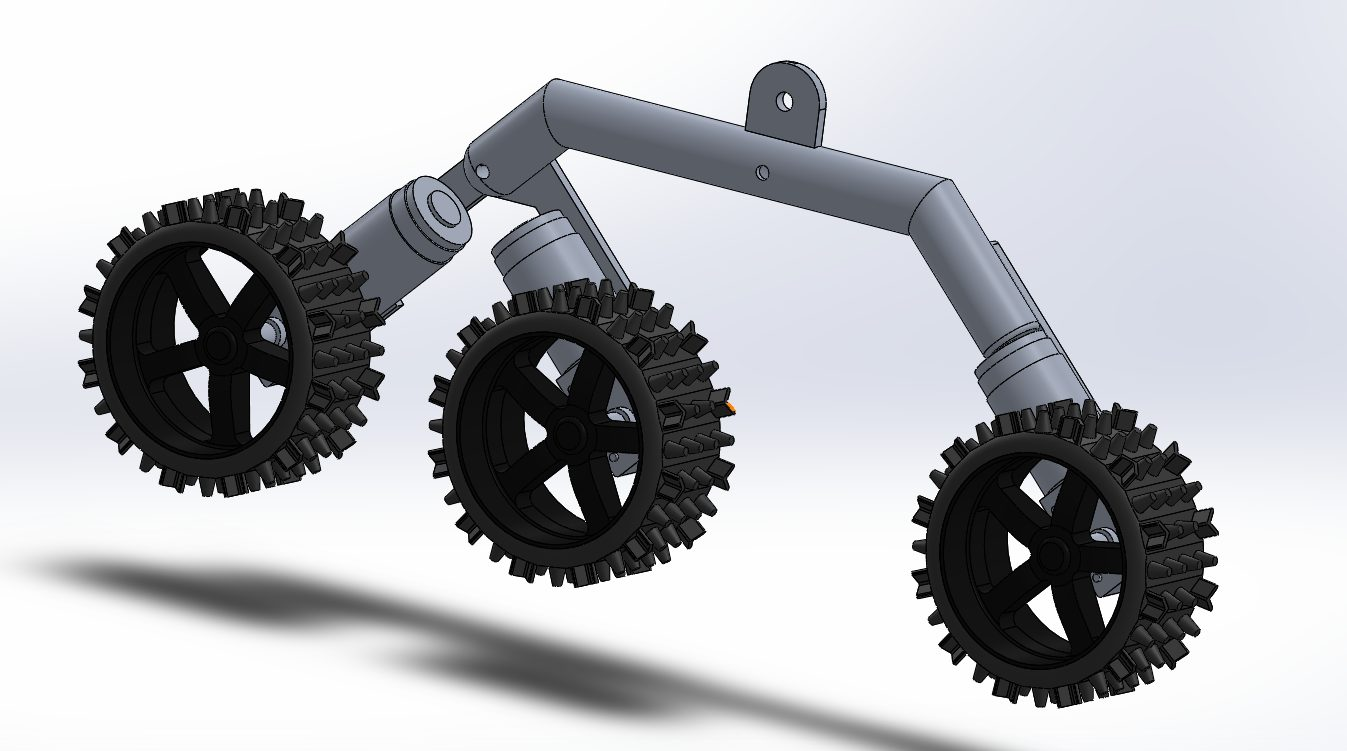
\includegraphics[width=0.2\textwidth]{images/suspensions/Rocker-Bogie Suspension.jpg}} \quad
    \subfloat[Multi-Link \cite{multilink_source}]{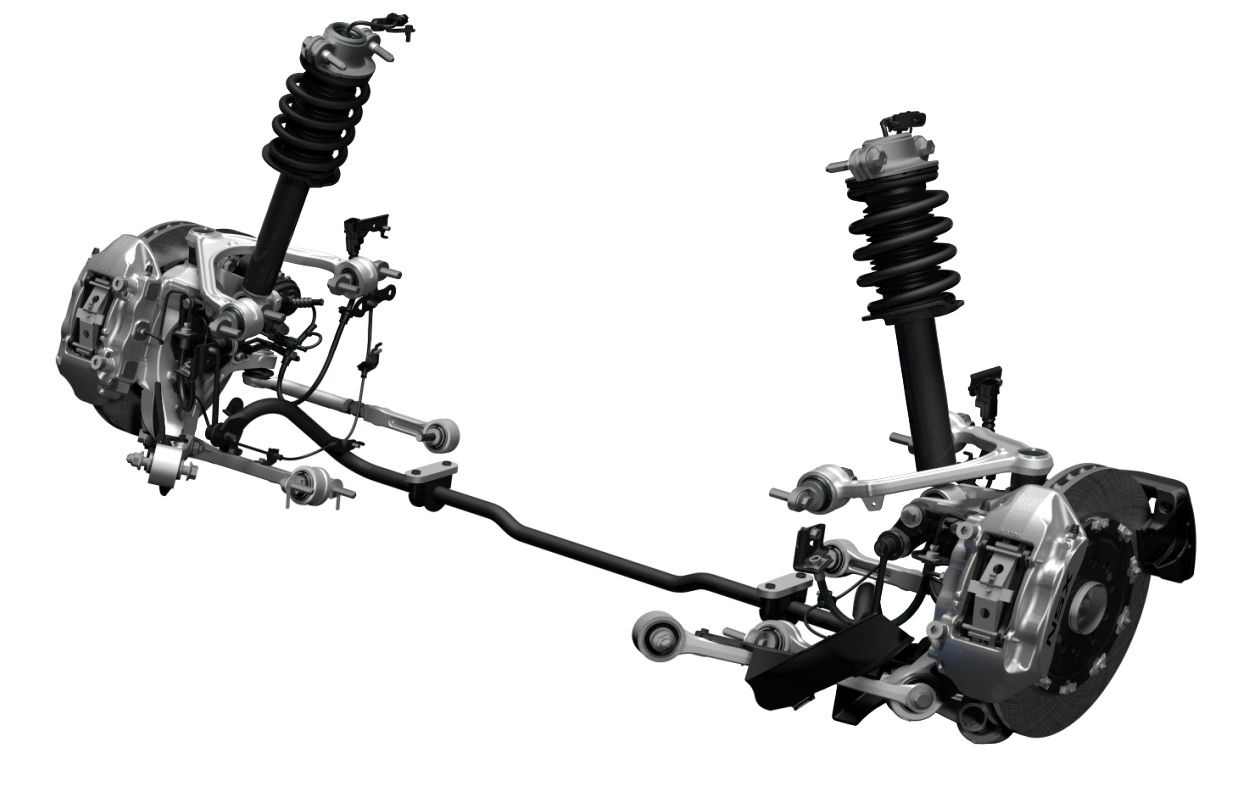
\includegraphics[width=0.2\textwidth]{images/suspensions/Multi-Link Suspension.jpg}} \\
    \subfloat[Articulated \cite{articulated_source}]{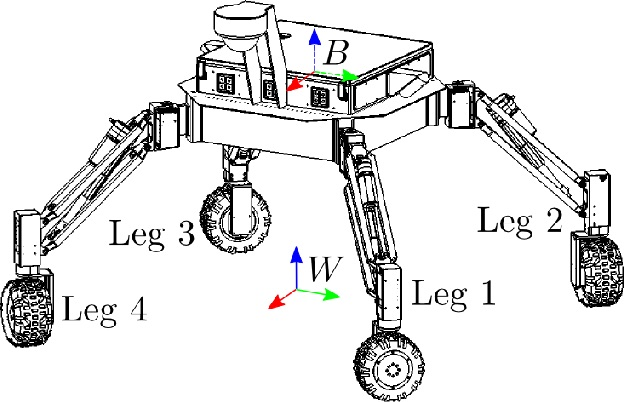
\includegraphics[width=0.2\textwidth]{images/suspensions/Articulated Suspension.jpg}} \quad
    \subfloat[Differential \cite{differential_source}]{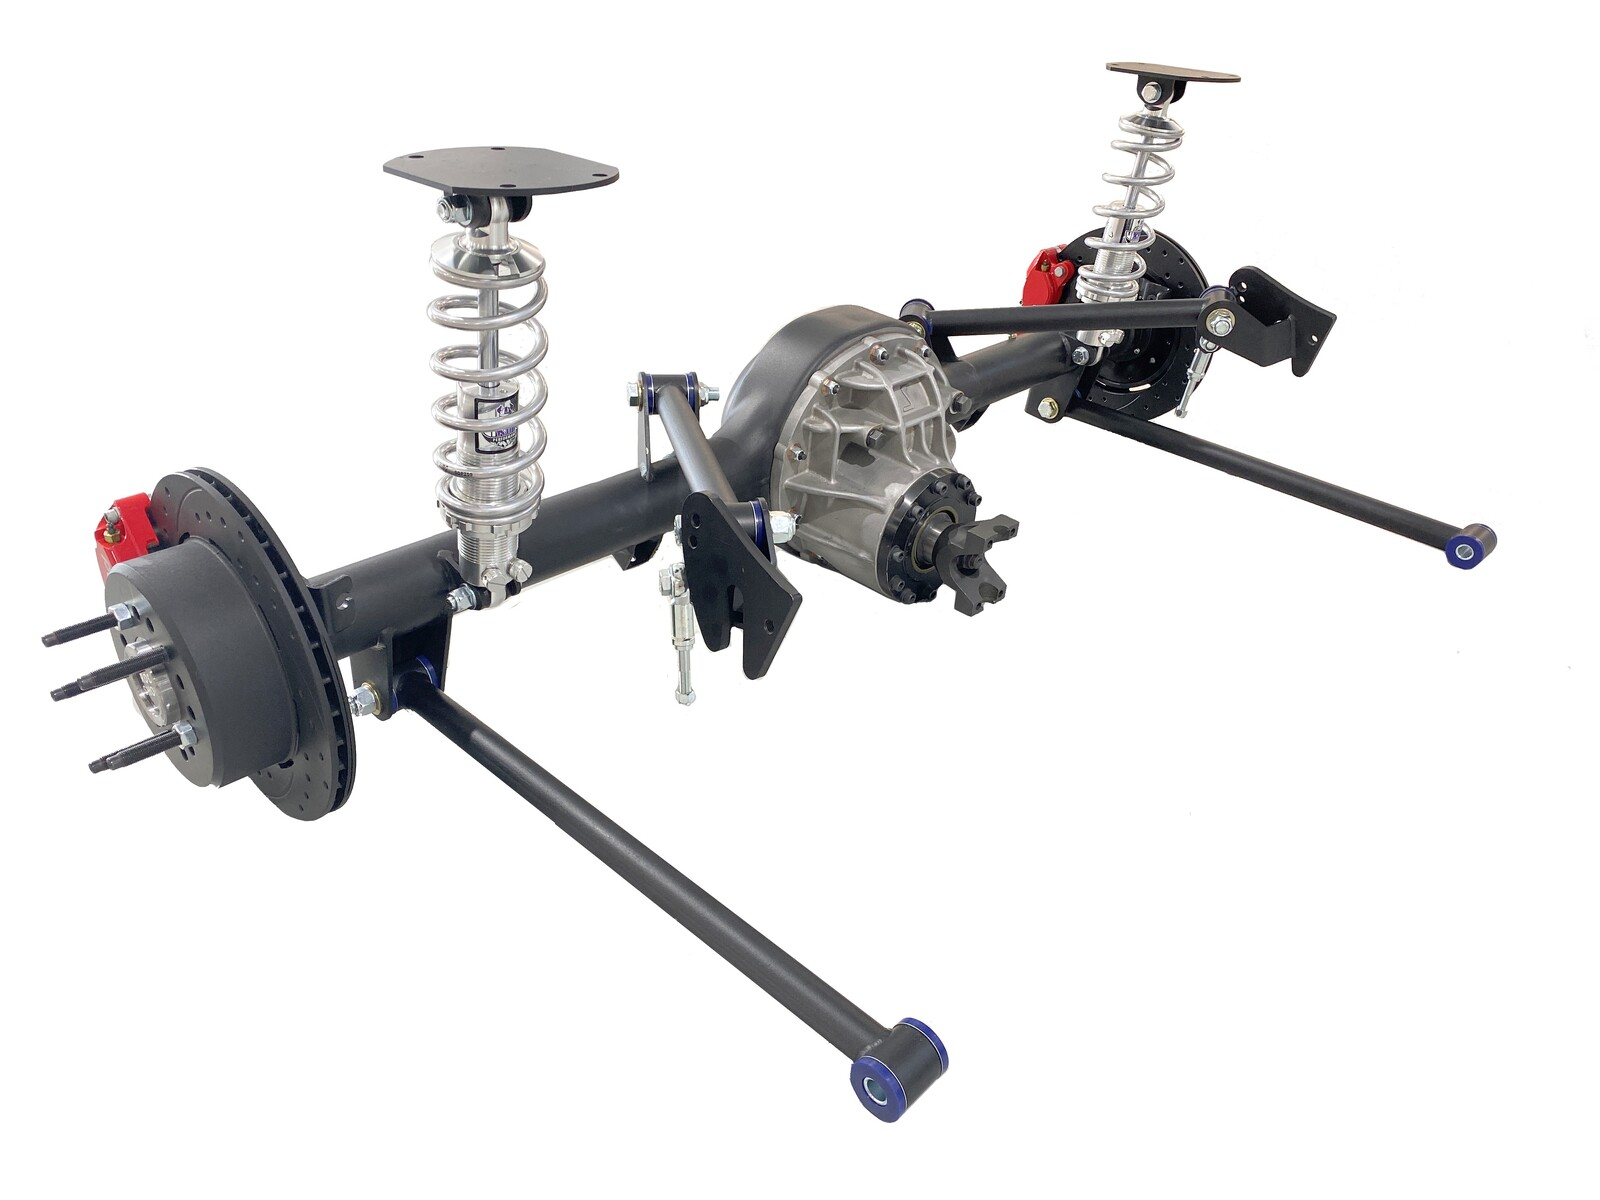
\includegraphics[width=0.2\textwidth]{images/suspensions/Differential Suspension.jpg}} \quad
    \subfloat[Leaf Spring \cite{leafspring_source}]{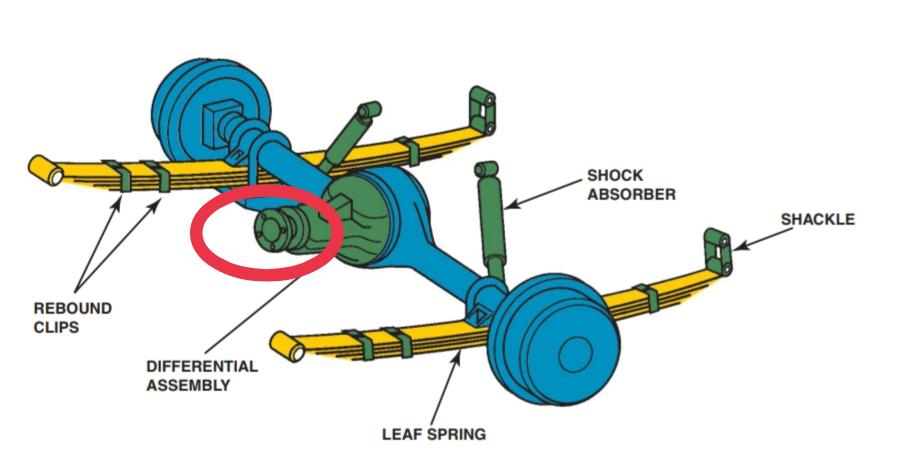
\includegraphics[width=0.2\textwidth]{images/suspensions/Leaf Spring Suspension.jpg}} \\
    \caption{Types of suspension systems in robotics.}
\end{figure}


\subsection{Vehicle-Inspired Suspension Designs}
Robotic suspension systems often draw inspiration from automobile engineering, adapting mechanical architectures to smaller and more agile platforms such as multi-link and spring-damper systems.
Conversely, rocker-bogie systems were originally designed for robotics but are influenced by mechanical linkages used in truck and railway bogie systems tailored for uneven tracks. 
On the same wavelength, leaf spring suspensions find the ideal environment in heavy-duty vehicles; due to that, they are preferred over other solutions in robotic contexts when cost and load capacity are the primary concerns over precision and agility. 
To sum up, these vehicle-inspired designs are particularly valuable for AMRs or robotics in general, where traditional robotic designs may not offer sufficient resilience or adaptability. 

\subsection{Existing AMR Suspension Solutions}
In the domain of AMRs, suspension designs vary significantly depending on the operating environment and task requirements. Many commercial AMRs operate in controlled indoor settings and thus may use rigid or minimal suspension systems. However, for heavy-duty AMRs designed to carry significant payloads or operate in semi-structured environments like warehouses, construction sites, or agriculture, more robust suspension systems are necessary.
Recent research and implementations show a growing trend toward hybrid and modular suspension systems. For instance, AMRs with spring-damper systems are becoming increasingly popular due to their balance of performance and simplicity. Platforms using articulated or bogie suspensions have also proven effective for navigating providing enhanced terrain compliance without requiring active control systems.
Despite these advancements, it remains a gap in affordable, high-performance suspension solutions tailored to medium and heavy-duty AMRs, particularly those that must operate in challenging environments while maintaining low production and maintenance costs. This motivates the exploration and development of novel or adapted suspension systems that prioritize both robustness and simplicity.

\newpage

\section{Concept Development}

\subsection{Design Constraints}
Given the nature of the AMR, the suspension system must be designed to withstand a variety of loads and conditions. The design constraints include:
\begin{itemize}
    \item \textbf{Load Capacity} \\ The suspension must support a maximum payload of 150 kg.
    \item \textbf{Terrain Adaptability} \\ The system should be capable of navigating uneven surfaces with obstacles taller than 10 mm.
    \item \textbf{Cost} \\ The total cost of the suspension system should not exceed €1000.
    \item \textbf{Maintenance} \\ The system should require minimal maintenance and be easy to repair or replace.
\end{itemize}

\vskip1em
Delving into the cost aspect, the suspension system must be designed to be cost-effective while still meeting performance requirements. The cost constraints include:
\begin{figure} [H]
    \centering
    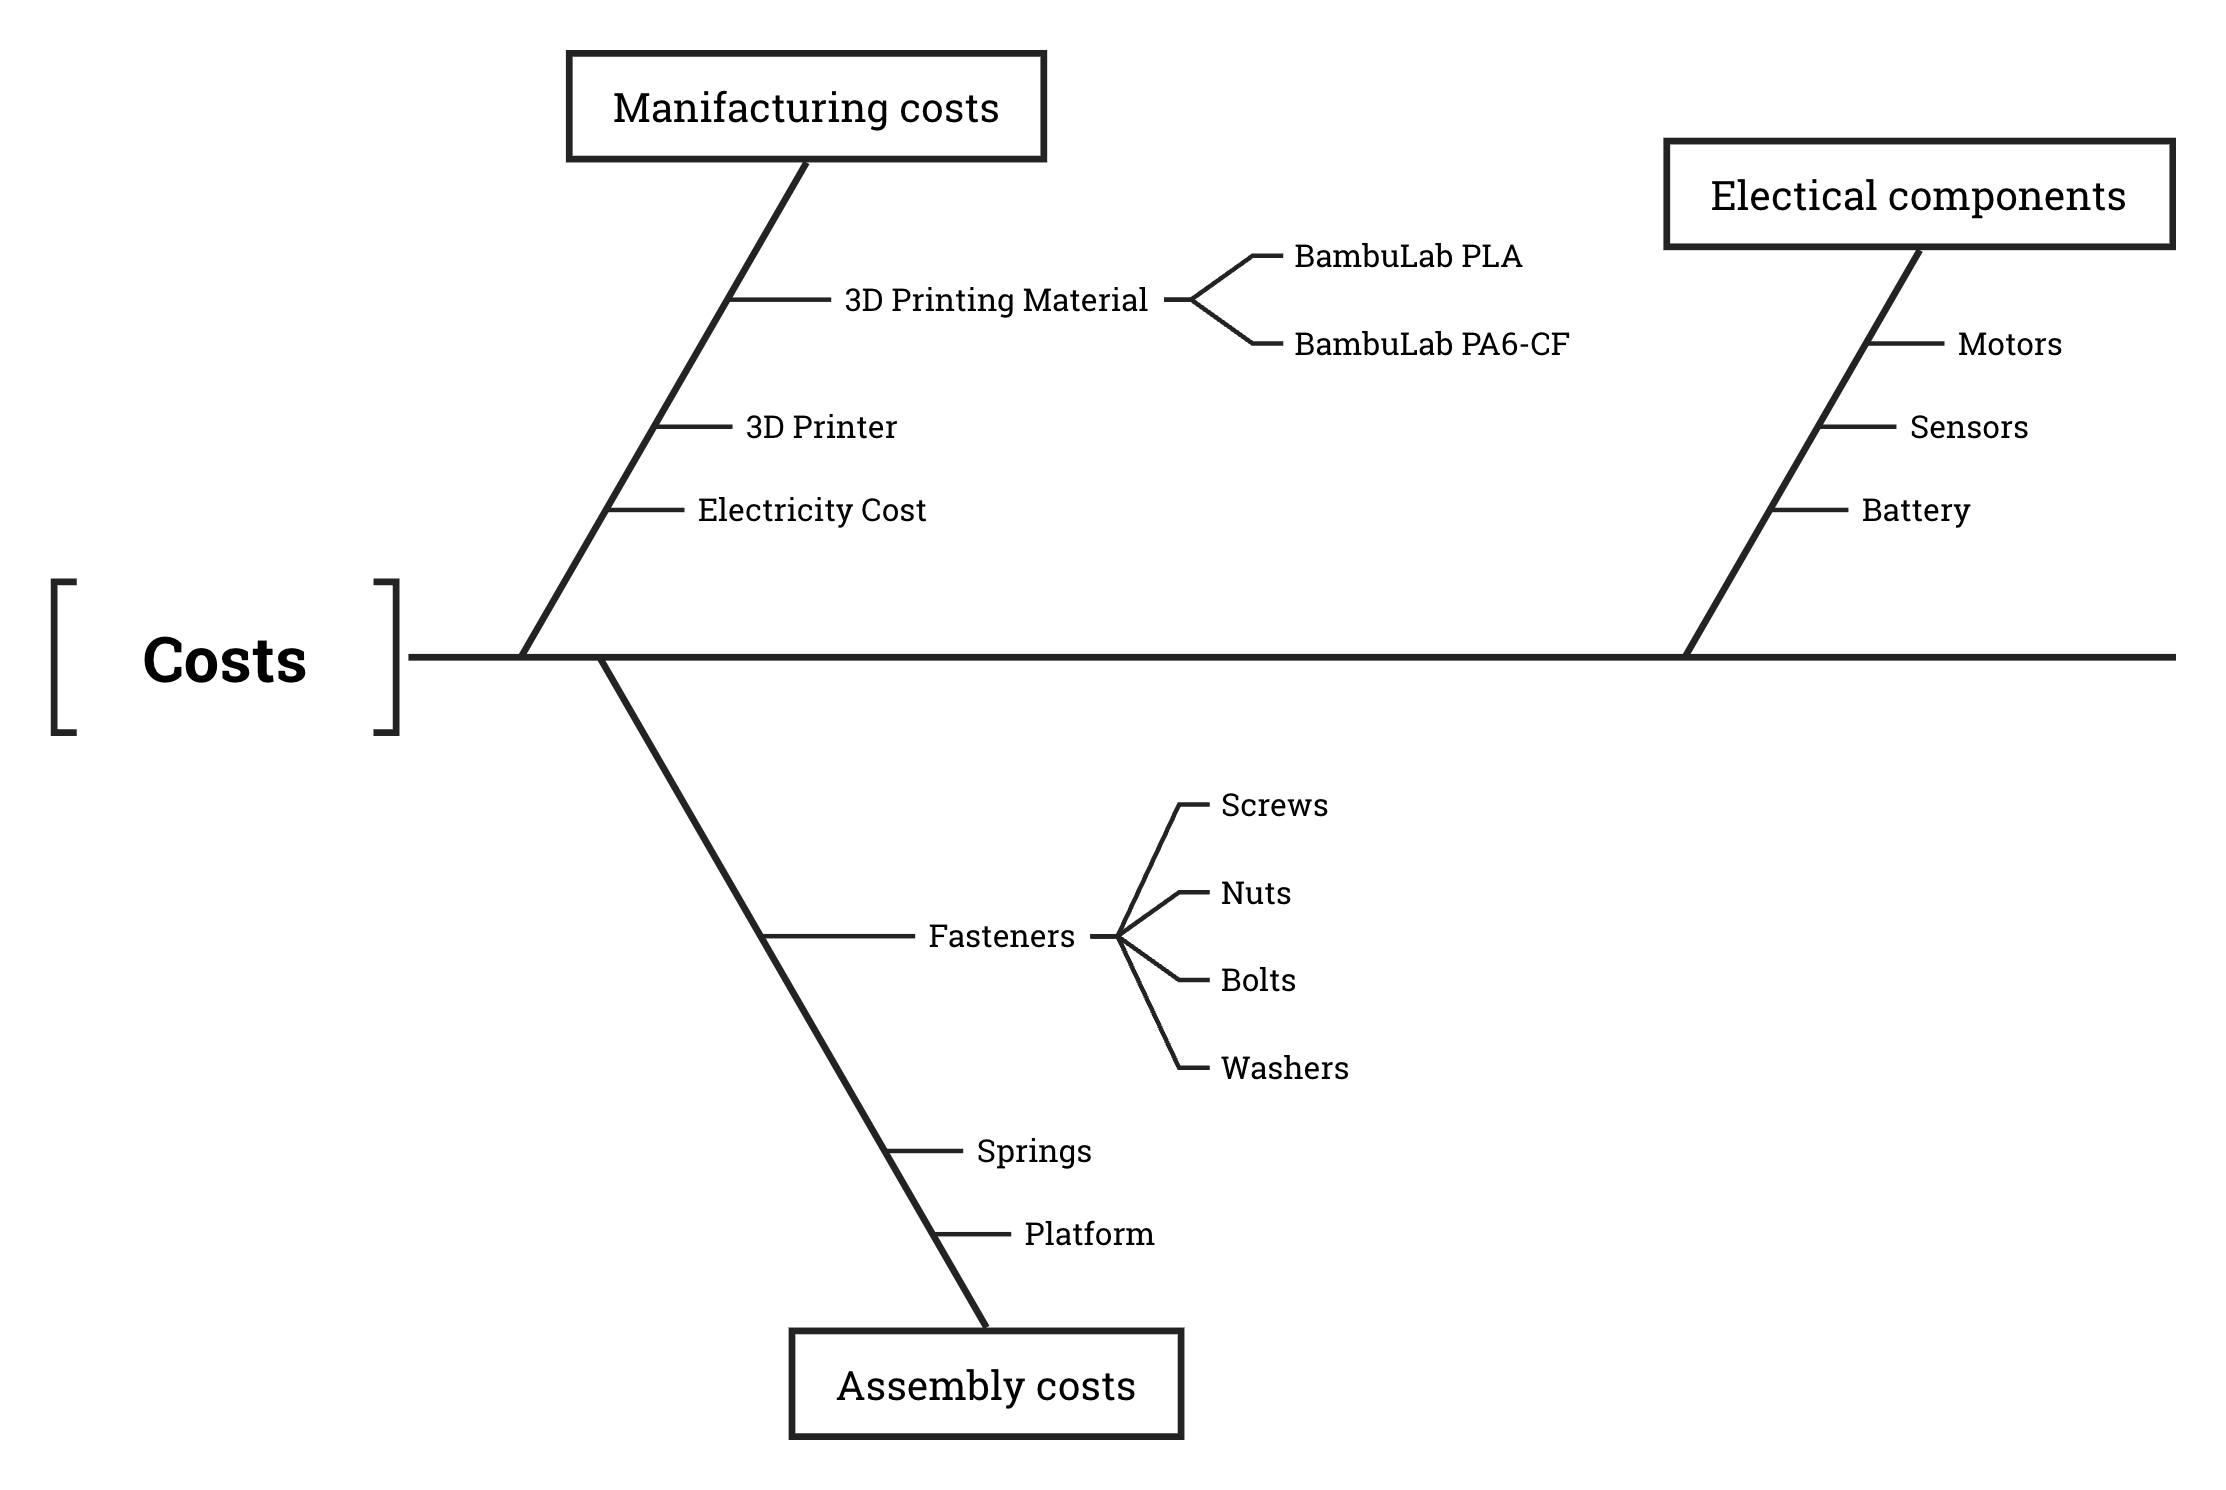
\includegraphics[width=0.8\textwidth]{images/Costs.png}
    \caption{Cost breakdown of the suspension system.}
    \label{fig:cost_breakdown}
    \caption*{The cost breakdown of the suspension system is divided into three main categories: materials, manufacturing, and assembly. The materials cost includes the price of the springs, dampers, and any additional components required for the suspension system. The manufacturing cost encompasses the expenses related to machining, welding, and other fabrication processes. Finally, the assembly cost covers labor and overhead associated with putting the suspension system together.}
\end{figure}

\newpage

\subsection{Trade-off Analysis}
Switching to the trade-off analysis, it is a systematic approach used to evaluate different design alternatives based on multiple criteria. This analysis took into account the original design born without the suspension system trying to figure out how to maximize the performance of the suspension system. In order to do that, a schematic representation of the suspension system idea has been created, which is shown in Figure \ref{fig:trade_off_analysis}:
\begin{figure}[H]
    \centering
    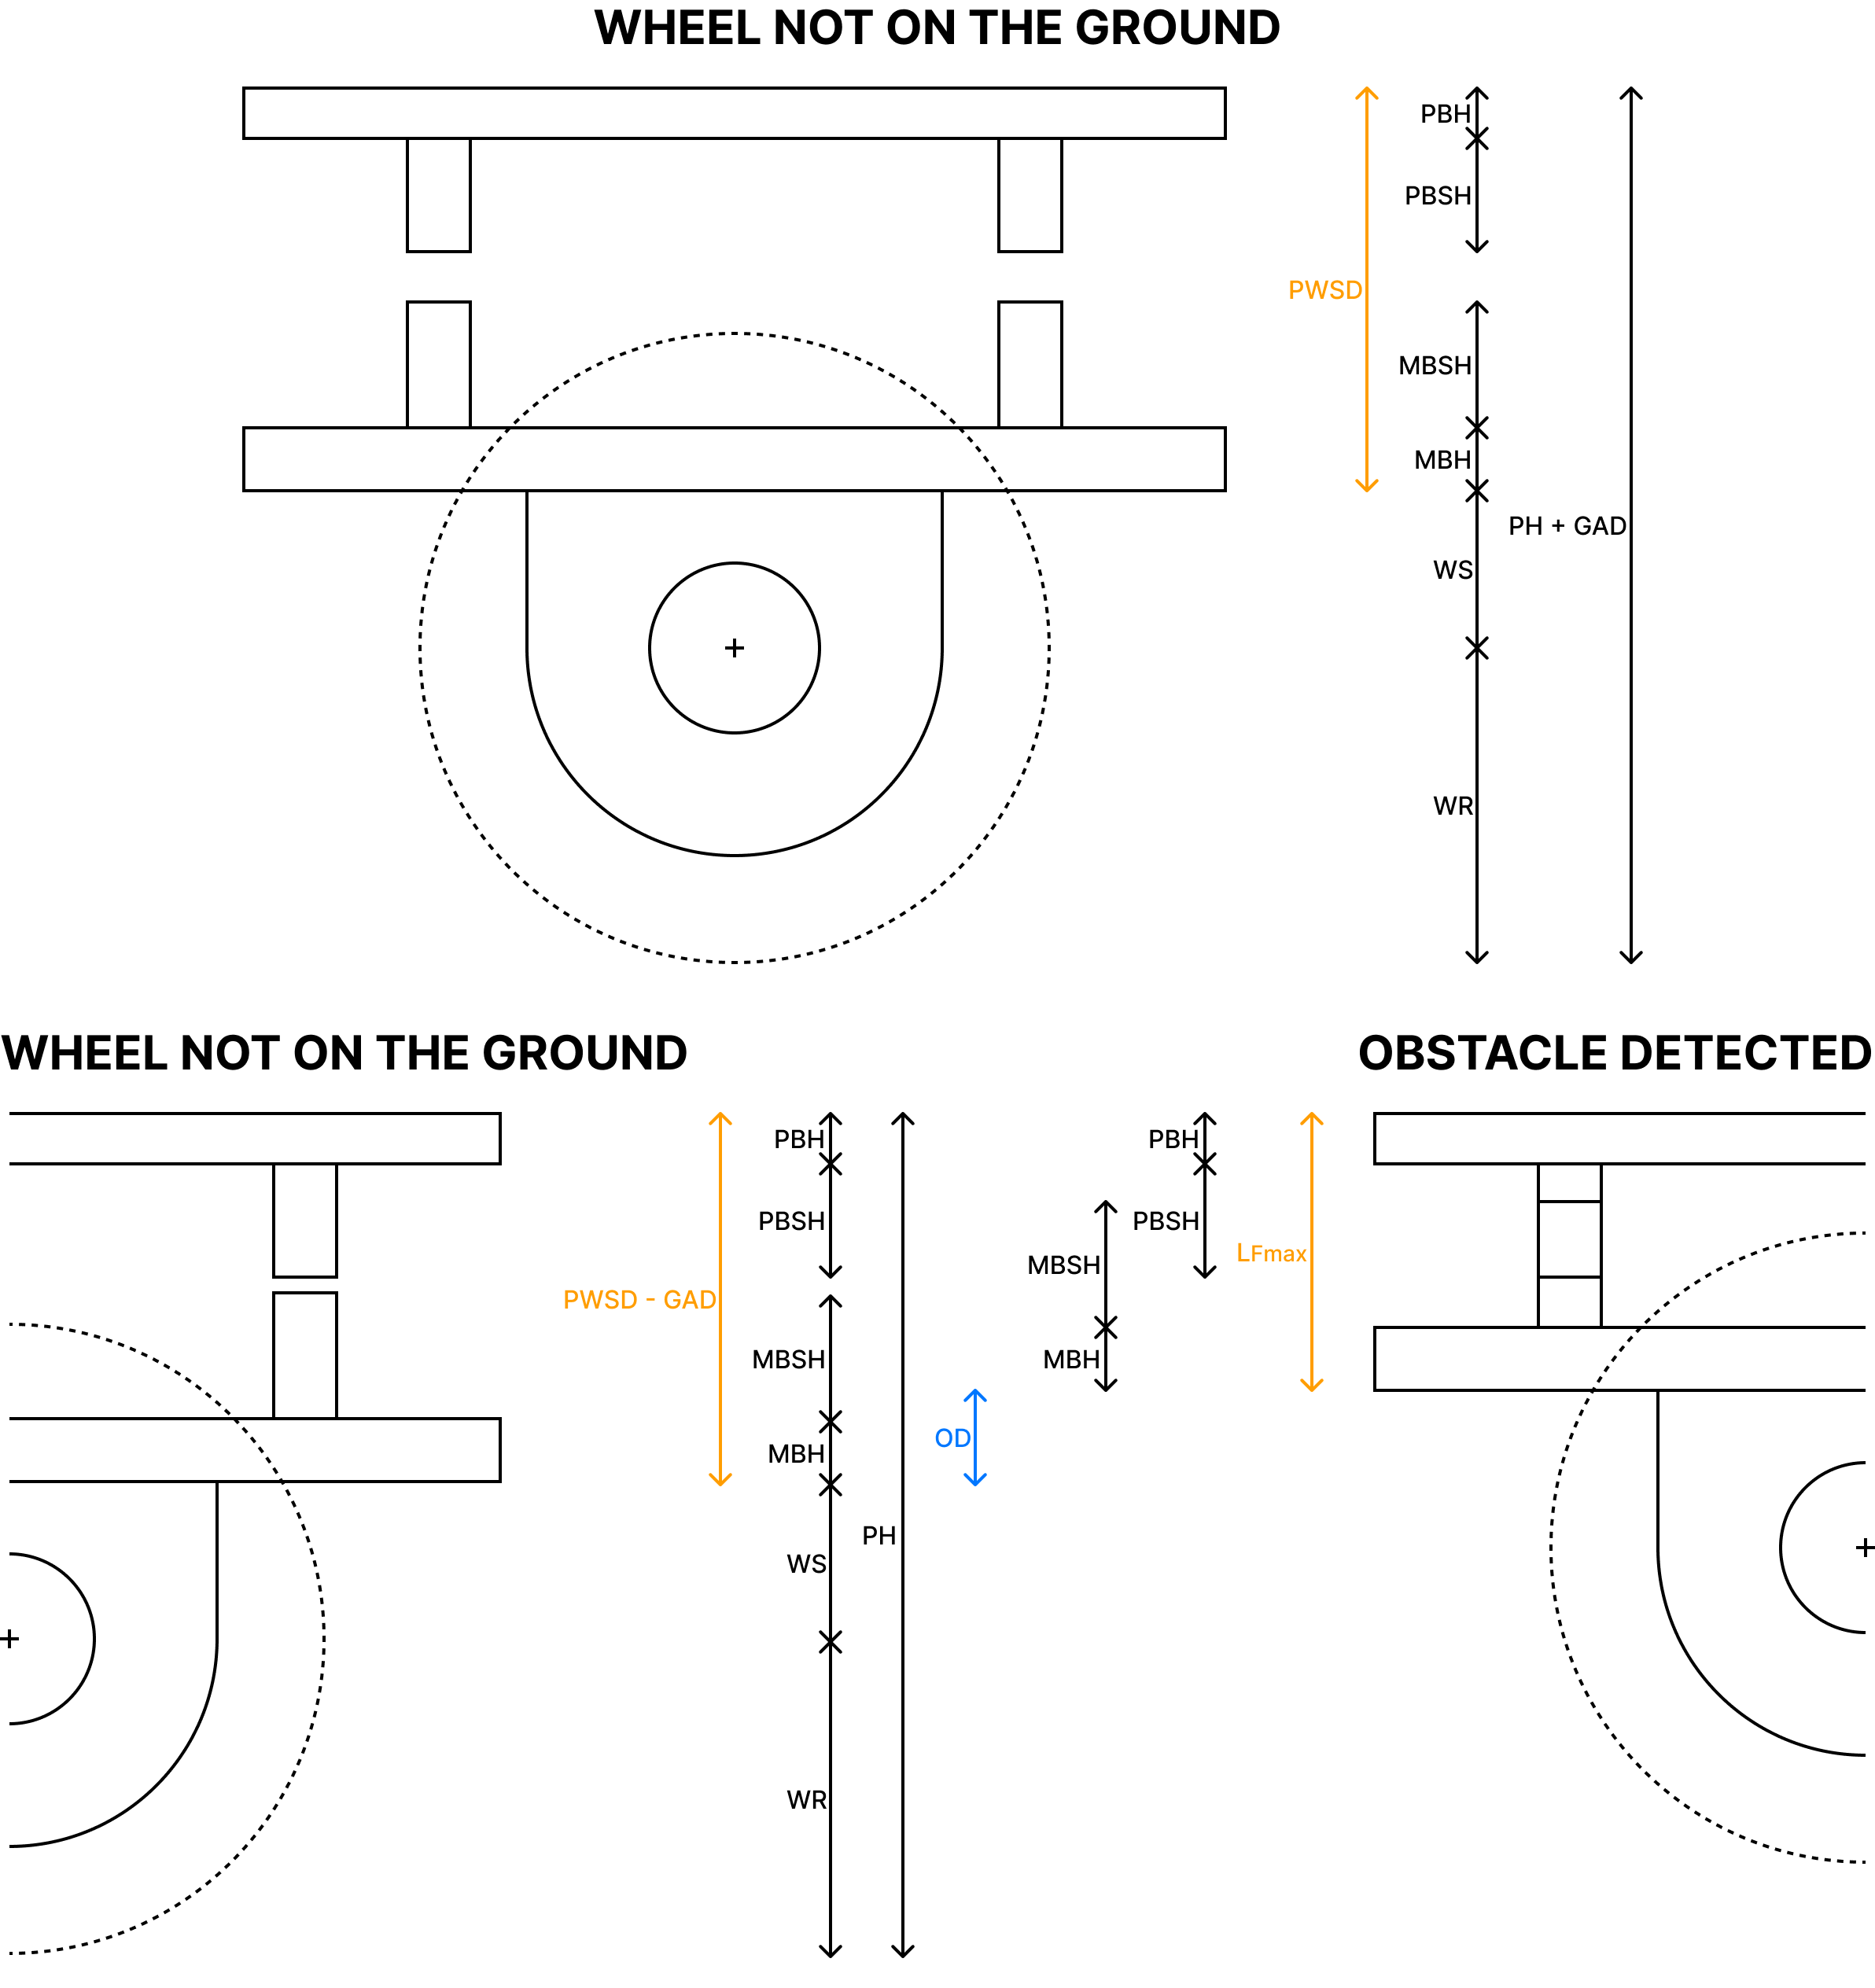
\includegraphics[width=\textwidth]{images/Trade-off Analysis.png}
    \caption{Trade-off analysis of the suspension system.}
    \label{fig:trade_off_analysis}
\end{figure}

\newpage
\noindent
The acronyms used in the figure are:
\begin{table}[H]
    \centering
    \begin{tabular}{|l|l|r|}
        \rowcolor{blue!5}
        \hline
        \textbf{Acronym} & \textbf{Description} & \textbf{Value} \\
        \hline
        PH    & Platform Height                  & 118 mm \\
        GAD   & Ground Adhesion Deflection       & 5 mm \\
        WR    & Wheel Radius                     & 50 mm \\
        WS    & Wheel Support                    & 25 mm \\
        MBH   & Motor Base Height                & 4 mm \\
        MBSH  & Motor Base Support Height        & 20 mm \\
        PBSH  & Platform Base Support Height     & 18 mm \\
        PBH   & Platform Base Height             & 2 mm \\
        PWSD  & Platform Wheel Support Distance  & -\\
        OD    & Obstacle Deflection              & -\\
        \hline
    \end{tabular}
    \caption{Acronyms used in the trade-off analysis.}
    \label{tab:trade_off_analysis_acronyms}
\end{table}

Being aware of the values of some of these parameters, it is possible to calculate the others in order to maximize the obstacle deflection. The following equations are used to calculate the parameters:
\begin{align}
    & \text{PWSD} = \text{PH} + \text{GAD} - \text{WR} - \text{WS} \\
    & \text{OD} = \text{PWSD} - \text{GAD} - L_ \text{Fmax}
\end{align}

Given the values of the parameters, it is possible to verify the following conditions in order to verify the geometry of the spring:
\begin{align}
    & \quad  L_0 \geq \text{PWSD} \\
    & \quad  L_\text{Fmax} - 2 \cdot \text{BH} \geq \text{PBSH} \\
    & \quad  L_\text{Fmax} - 2 \cdot \text{BH} \geq \text{MBSH}
\end{align}

\newpage

\subsection{Spring Component}
The suspension system is composed of several key components, each designed to fulfill specific functions and requirements.

The spring is a critical component of the suspension system, providing the necessary force to support the AMR's weight and absorb shocks from uneven terrain. The spring is designed to be adjustable in terms of length and stiffness, allowing for customization based on the AMR's payload and operating conditions.

In order to figure that out, a parametric design has been created to be able to change the parameters of the spring easily and quickly. To carry out this purpose, a Python algorithm (already available on
the GitHub repository \cite{github_repository}) has been developed to calculate the spring parameters based on the input values and verify the conditions needed to be satisfied (as mentioned in the following section).

Despite the vital importance of a well-structured algorithm, it is equally important to rely on a good database of springs that enables the selection of the right spring for the AMR. The database choosen is the one provided by \textit{Molle Industriali} \cite{molle_industriali_source}, a robust spring manufacturer that provides a wide range of springs for different applications.

Given this preamble regarding the sources and the tools involved in the design of the spring, it is possible to highlight the recommended springs for the AMR based on the payload:

\begin{table}[H]
    \centering
    \resizebox{\textwidth}{!}{
    \begin{tabular}{|c|c|c|c|c|c|c|c|c|c|c|c|}
    \rowcolor{blue!5}
        \hline
        \textbf{Payload [kg]} & \textbf{Material} & \textbf{$d$ [mm]} & \textbf{$D$ [mm]} & \textbf{$L_0$ [mm]} & \textbf{$L_\text{Fmax}$ [mm]} & \textbf{$k$ [N/m]} & \textbf{$\text{CS}_\text{sta}$} & \textbf{$\text{CS}_\text{fat}$} & \textbf{$f_\text{ost}$ [mm]} & \textbf{$i_\text{eff}$} & \textbf{Code} \\
        \hline
        10 & Filo di acciaio armonico & 1.07 & 8.07 & 50.80 & 27.20 & 1.80 & 2.96 & 1.90 & 15.80 & 14.03 & \href{https://www.molle-industriali.it/C03600422000M}{C03600422000M} \\
        26 & Acciaio inossidabile 302 & 1.30 & 10.89 & 50.80 & 26.09 & 1.88 & 1.74 & 1.10 & 16.91 & 10.88 & \href{https://www.molle-industriali.it/C04800512000S}{C04800512000S} \\
        41 & Acciaio inossidabile 316 & 1.30 & 10.89 & 50.80 & 26.09 & 1.88 & 1.19 & 1.10 & 16.91 & 10.88 & \href{https://www.molle-industriali.it/C04800512000S}{C04800512000S} \\
        57 & Acciaio zincato & 1.30 & 10.89 & 50.80 & 26.09 & 2.26 & 1.12 & 1.09 & 16.91 & 9.91 & \href{https://www.molle-industriali.it/C04800512000M}{C04800512000M} \\
        72 & Filo di acciaio armonico & 1.88 & 22.89 & 50.80 & 26.95 & 2.26 & 1.36 & 2.27 & 16.05 & 4.67 & \href{https://www.molle-industriali.it/C09750742000M}{C09750742000M} \\
        88 & Filo di acciaio armonico & 1.88 & 22.89 & 50.80 & 26.95 & 2.26 & 1.14 & 2.27 & 16.05 & 4.67 & \href{https://www.molle-industriali.it/C09750742000M}{C09750742000M} \\
        103 & Acciaio inossidabile 302 & 2.16 & 25.78 & 50.80 & 27.51 & 2.54 & 1.07 & 1.45 & 15.49 & 4.63 & \href{https://www.molle-industriali.it/C11000852000S}{C11000852000S} \\
        119 & Filo di acciaio armonico & 2.16 & 25.78 & 50.80 & 27.51 & 3.05 & 1.16 & 1.56 & 15.49 & 4.22 & \href{https://www.molle-industriali.it/C11000852000M}{C11000852000M} \\
        134 & Acciaio inossidabile 302 & 2.44 & 28.68 & 50.80 & 28.02 & 3.28 & 1.08 & 1.15 & 14.98 & 4.24 & \href{https://www.molle-industriali.it/C12250962000S}{C12250962000S} \\
        150 & Filo di acciaio armonico & 2.44 & 28.68 & 50.80 & 28.02 & 3.94 & 1.20 & 1.33 & 14.98 & 3.86 & \href{https://www.molle-industriali.it/C12250962000M}{C12250962000M} \\
        \hline
    \end{tabular}
    }
    \caption{Springs for parametric design}
    \label{tab:spring_parametric_design}
\end{table}

\newpage

\subsection{CAD Model Overview}
The CAD model of the suspension system was developed using Fusion360, a powerful CAD software that allows for parametric design and simulation within the ANSYS environment. The model includes all components of the suspension system, including the spring and all the components that are needed to assemble the suspension system liking the chassis and the wheels. The model is designed to be easily adjustable, allowing for quick modifications to parameters such as spring length, diameter, and material properties. This flexibility is crucial for optimizing the suspension system's performance based on the specific requirements of the AMR.

\begin{figure}[H]
    \centering
    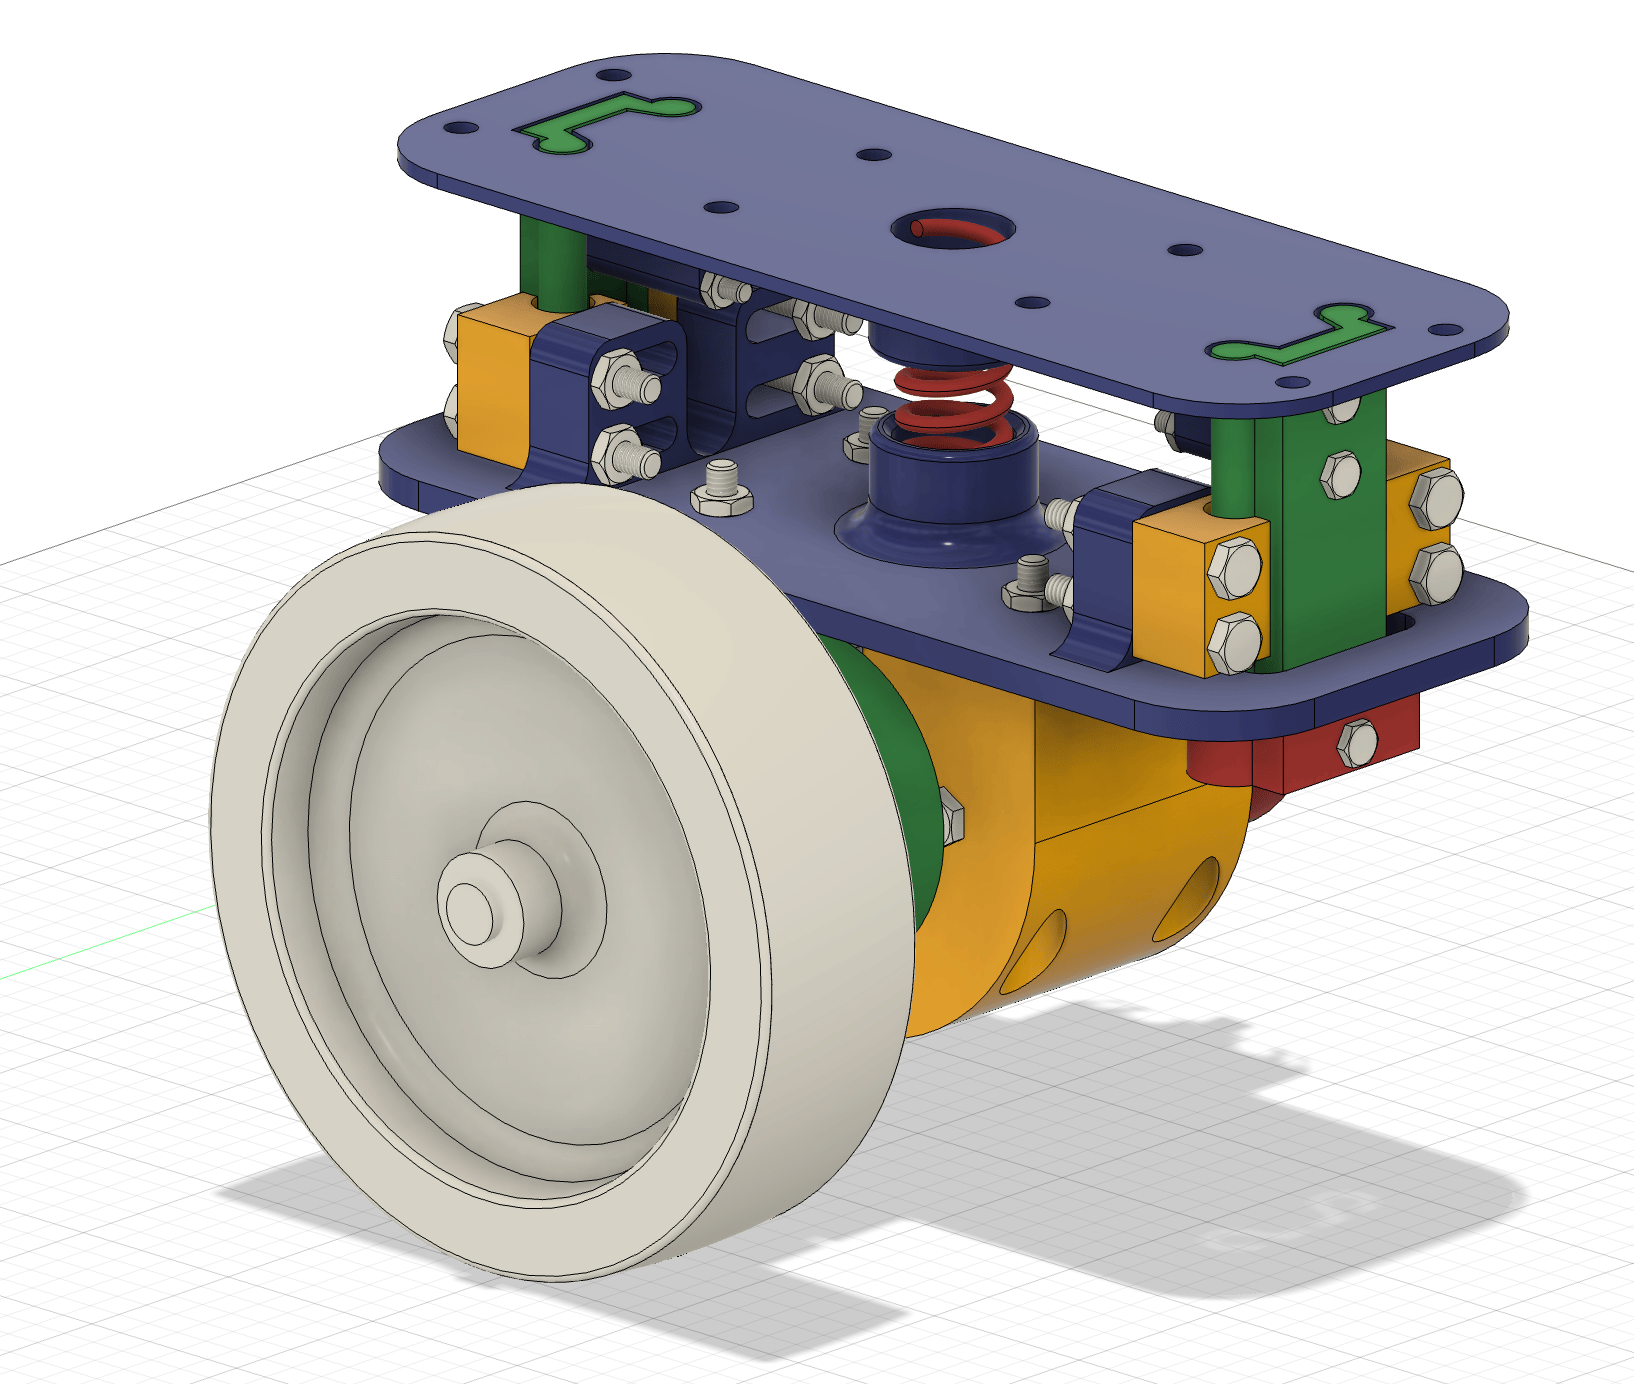
\includegraphics[width=\textwidth]{images/CAD design/Suspension.png}
    \caption{CAD model of the suspension system}
    \label{fig:cad_model}
\end{figure}

\newpage
Based on the figure \ref{fig:cad_model}, it is possible to highlight the main components of the suspension system as:
\begin{table}[H]
    \centering
    \resizebox{\textwidth}{!}{
    \begin{tabular}[t]{@{}m{0.4\textwidth} m{0.6\textwidth}@{}}
        \begin{minipage}[t]{\linewidth}
        \vspace{0pt}
        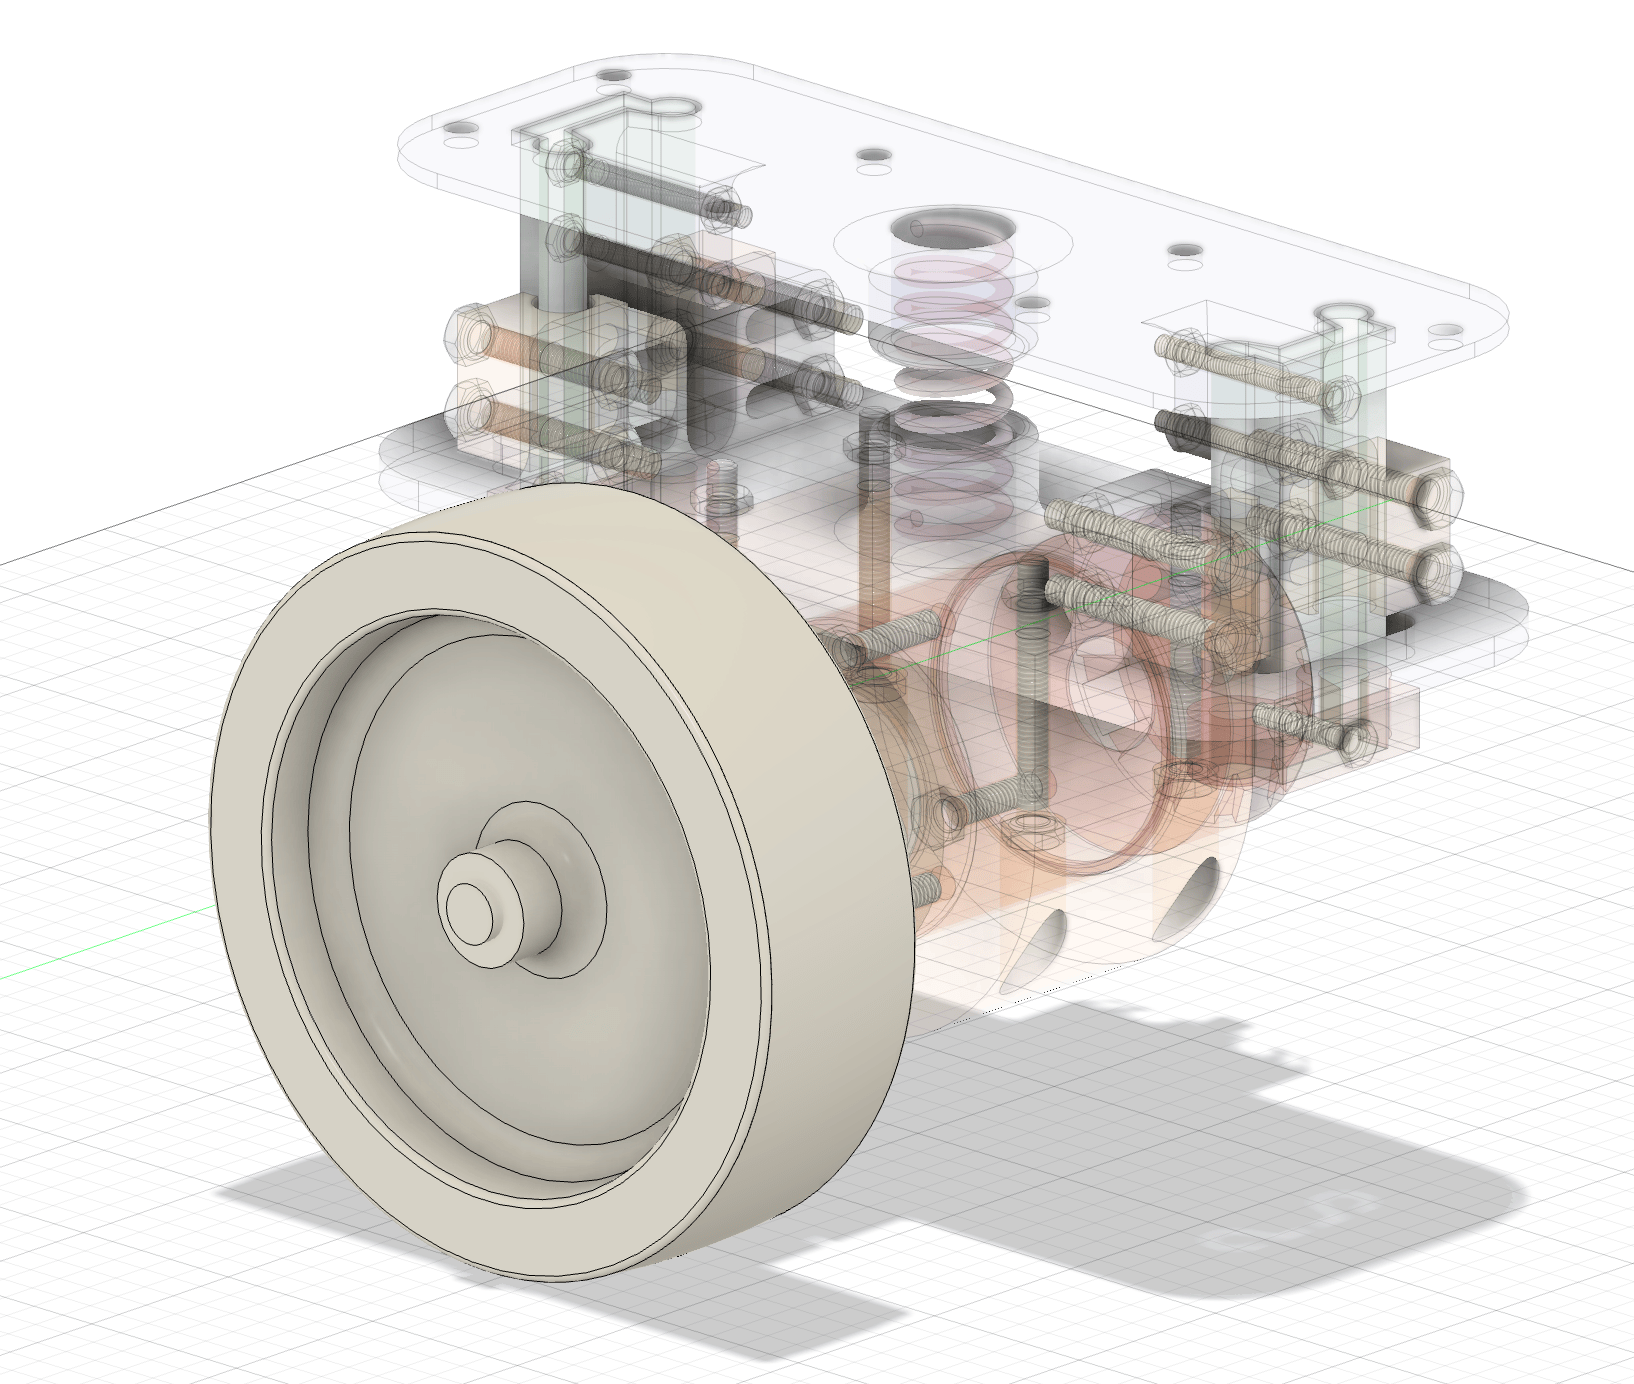
\includegraphics[width=\textwidth]{images/CAD design/Wheel.png}
        \end{minipage}
        &
        \begin{minipage}[t]{\linewidth}
        \vspace{0pt}
        \textbf{Wheel} \\ The wheel is a vital component of the suspension system, providing the necessary contact with the ground and enabling movement. The main requirements for the wheel is to be sufficiently rigid and to possess a high grip on the ground.
        \end{minipage}
        \\
    \end{tabular}}
\end{table}

\begin{table}[H]
    \centering
    \resizebox{\textwidth}{!}{
    \begin{tabular}[t]{@{}m{0.4\textwidth} m{0.6\textwidth}@{}}
        \begin{minipage}[t]{\linewidth}
        \vspace{0pt}
        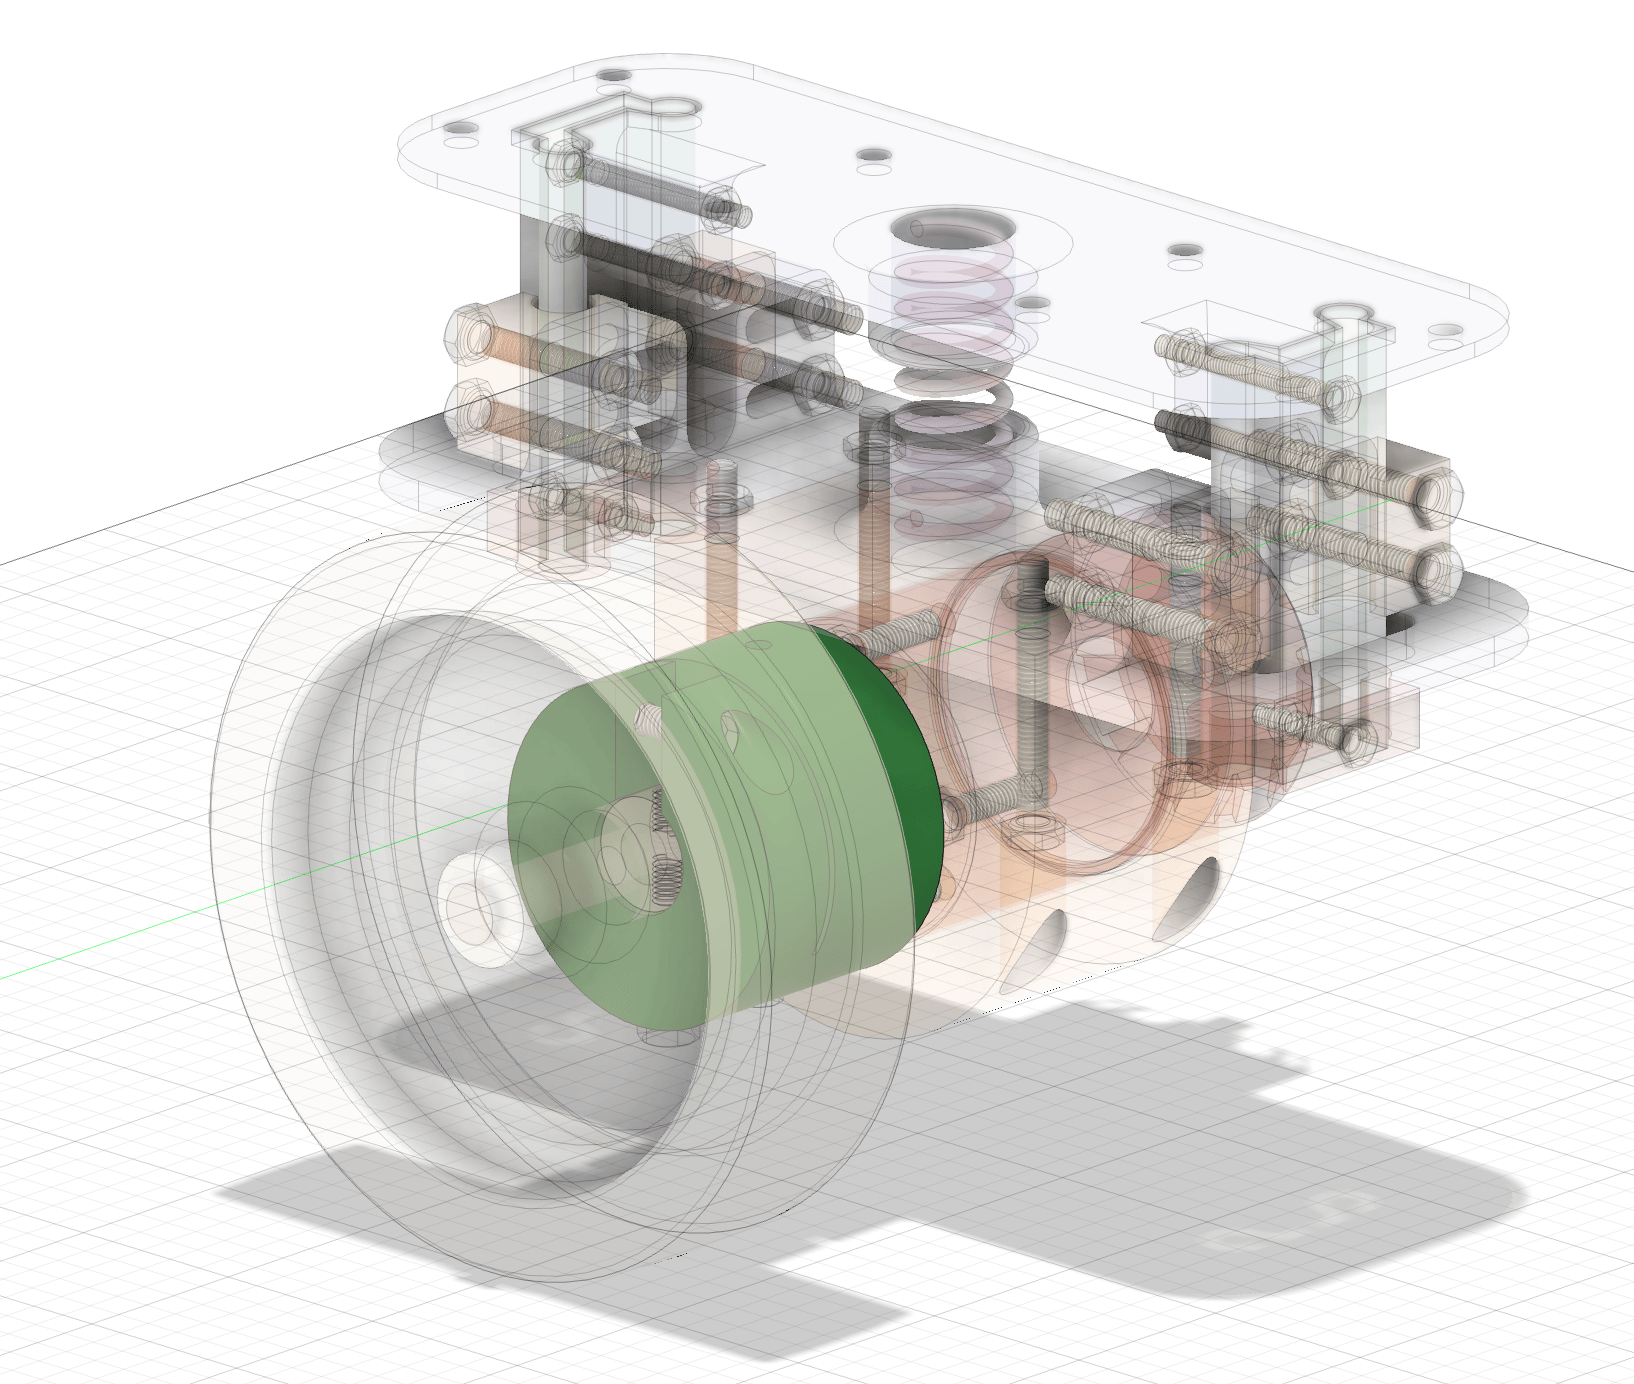
\includegraphics[width=\textwidth]{images/CAD design/Adaptor.png}
        \end{minipage}
        &
        \begin{minipage}[t]{\linewidth}
        \vspace{0pt}
        \textbf{Adaptor} \\ The adaptor wheel-motor is a crucial component that connects the wheels to the motor, allowing for efficient power transfer and control. It is designed to withstand the forces generated during operation trying to avoid as much as possible situations in which components such as screws work on shear.
        \end{minipage}
        \\
    \end{tabular}}
\end{table}

\begin{table}[H]
    \centering
    \resizebox{\textwidth}{!}{
    \begin{tabular}[t]{@{}m{0.4\textwidth} m{0.6\textwidth}@{}}
        \begin{minipage}[t]{\linewidth}
        \vspace{0pt}
        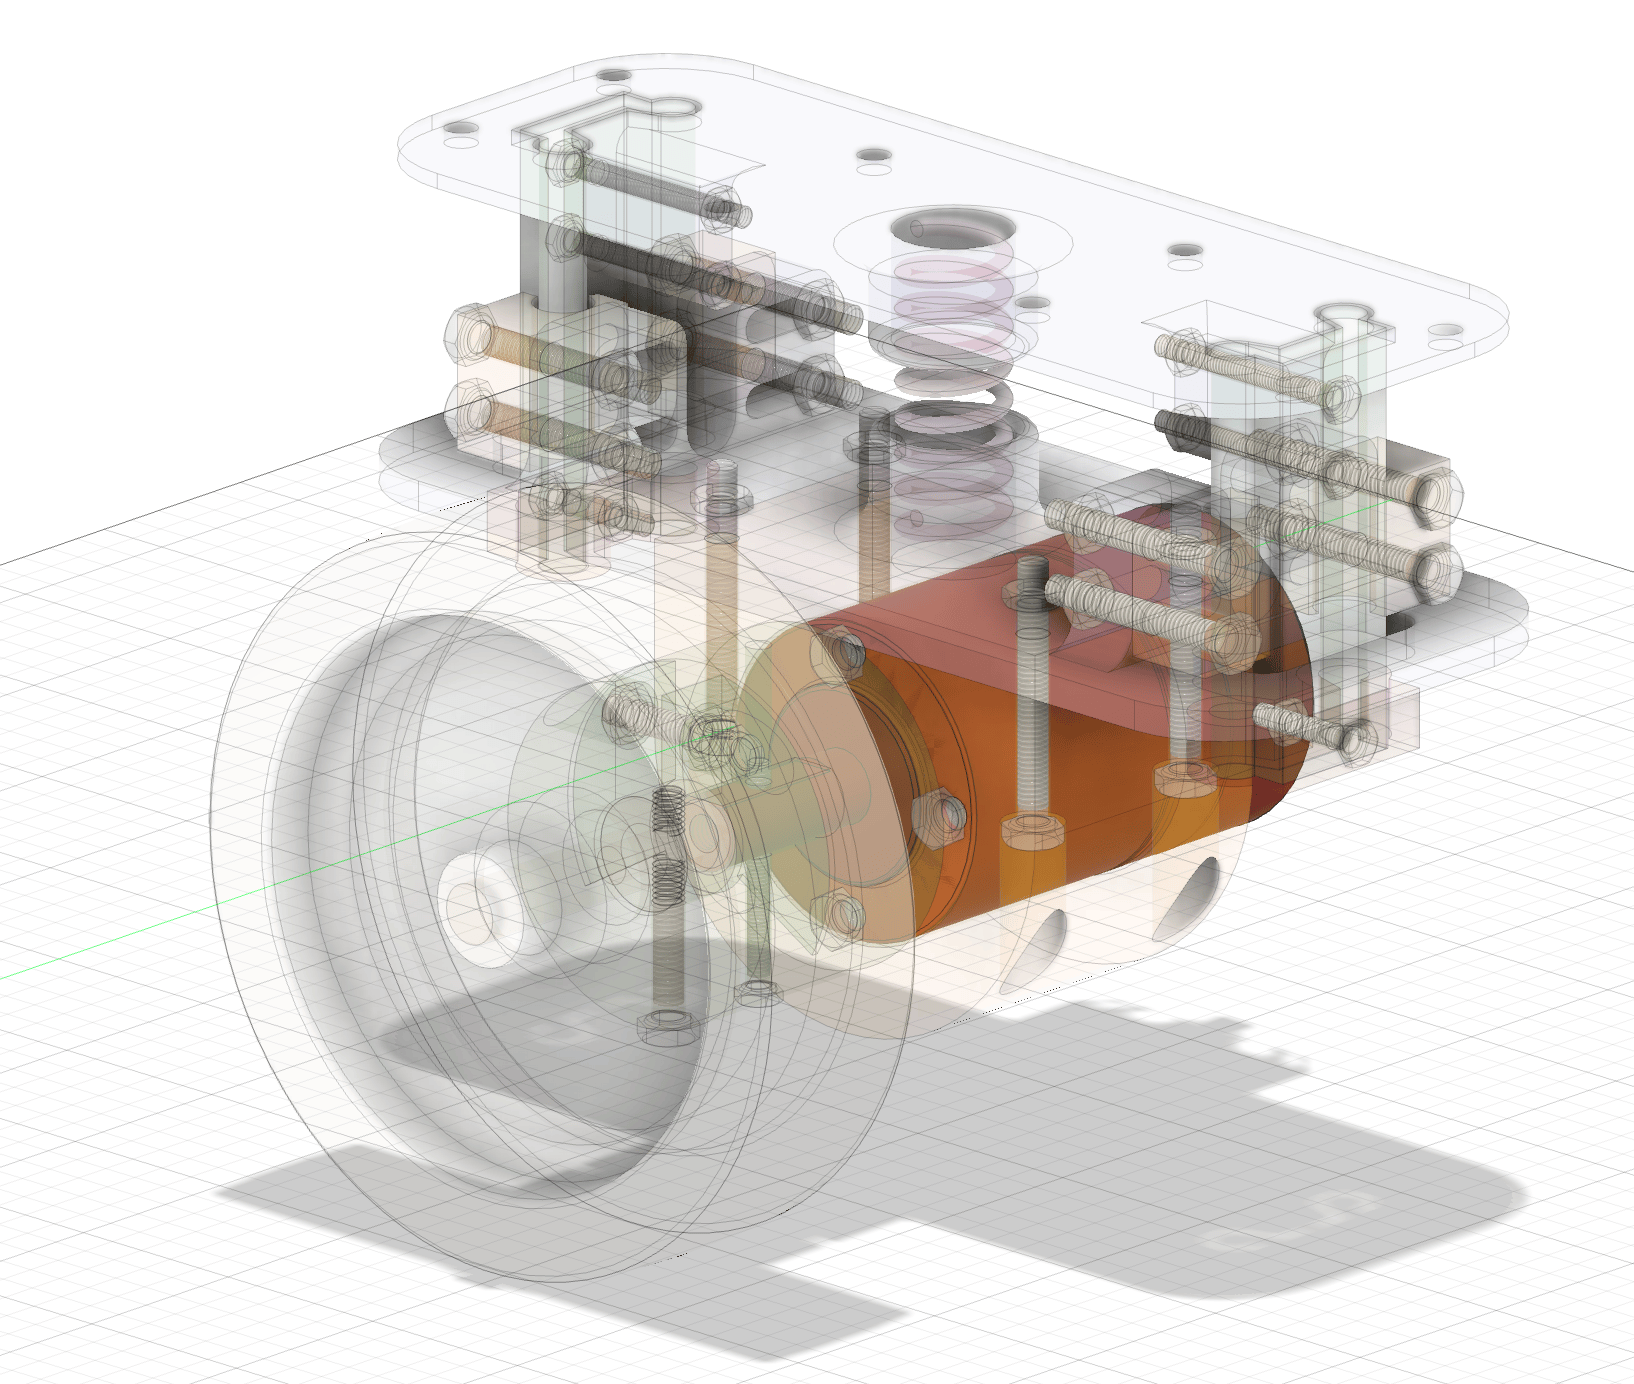
\includegraphics[width=\textwidth]{images/CAD design/Motor.png}
        \end{minipage}
        &
        \begin{minipage}[t]{\linewidth}
        \vspace{0pt}
        \textbf{Motor} \\ The motor is a critical component of the suspension system, providing the necessary power to drive the wheels and control the AMR's movement. It has been choosen to be lightweight and compact, allowing for easy integration into the overall system allowing to provide the necessary torque and speed for the AMR's intended applications. The motor is designed to be easily replaceable, ensuring minimal downtime in case of failure.
        \end{minipage}
        \\
    \end{tabular}}
\end{table}

\begin{table}[H]
    \centering
    \resizebox{\textwidth}{!}{
    \begin{tabular}[t]{@{}m{0.4\textwidth} m{0.6\textwidth}@{}}
        \begin{minipage}[t]{\linewidth}
        \vspace{0pt}
        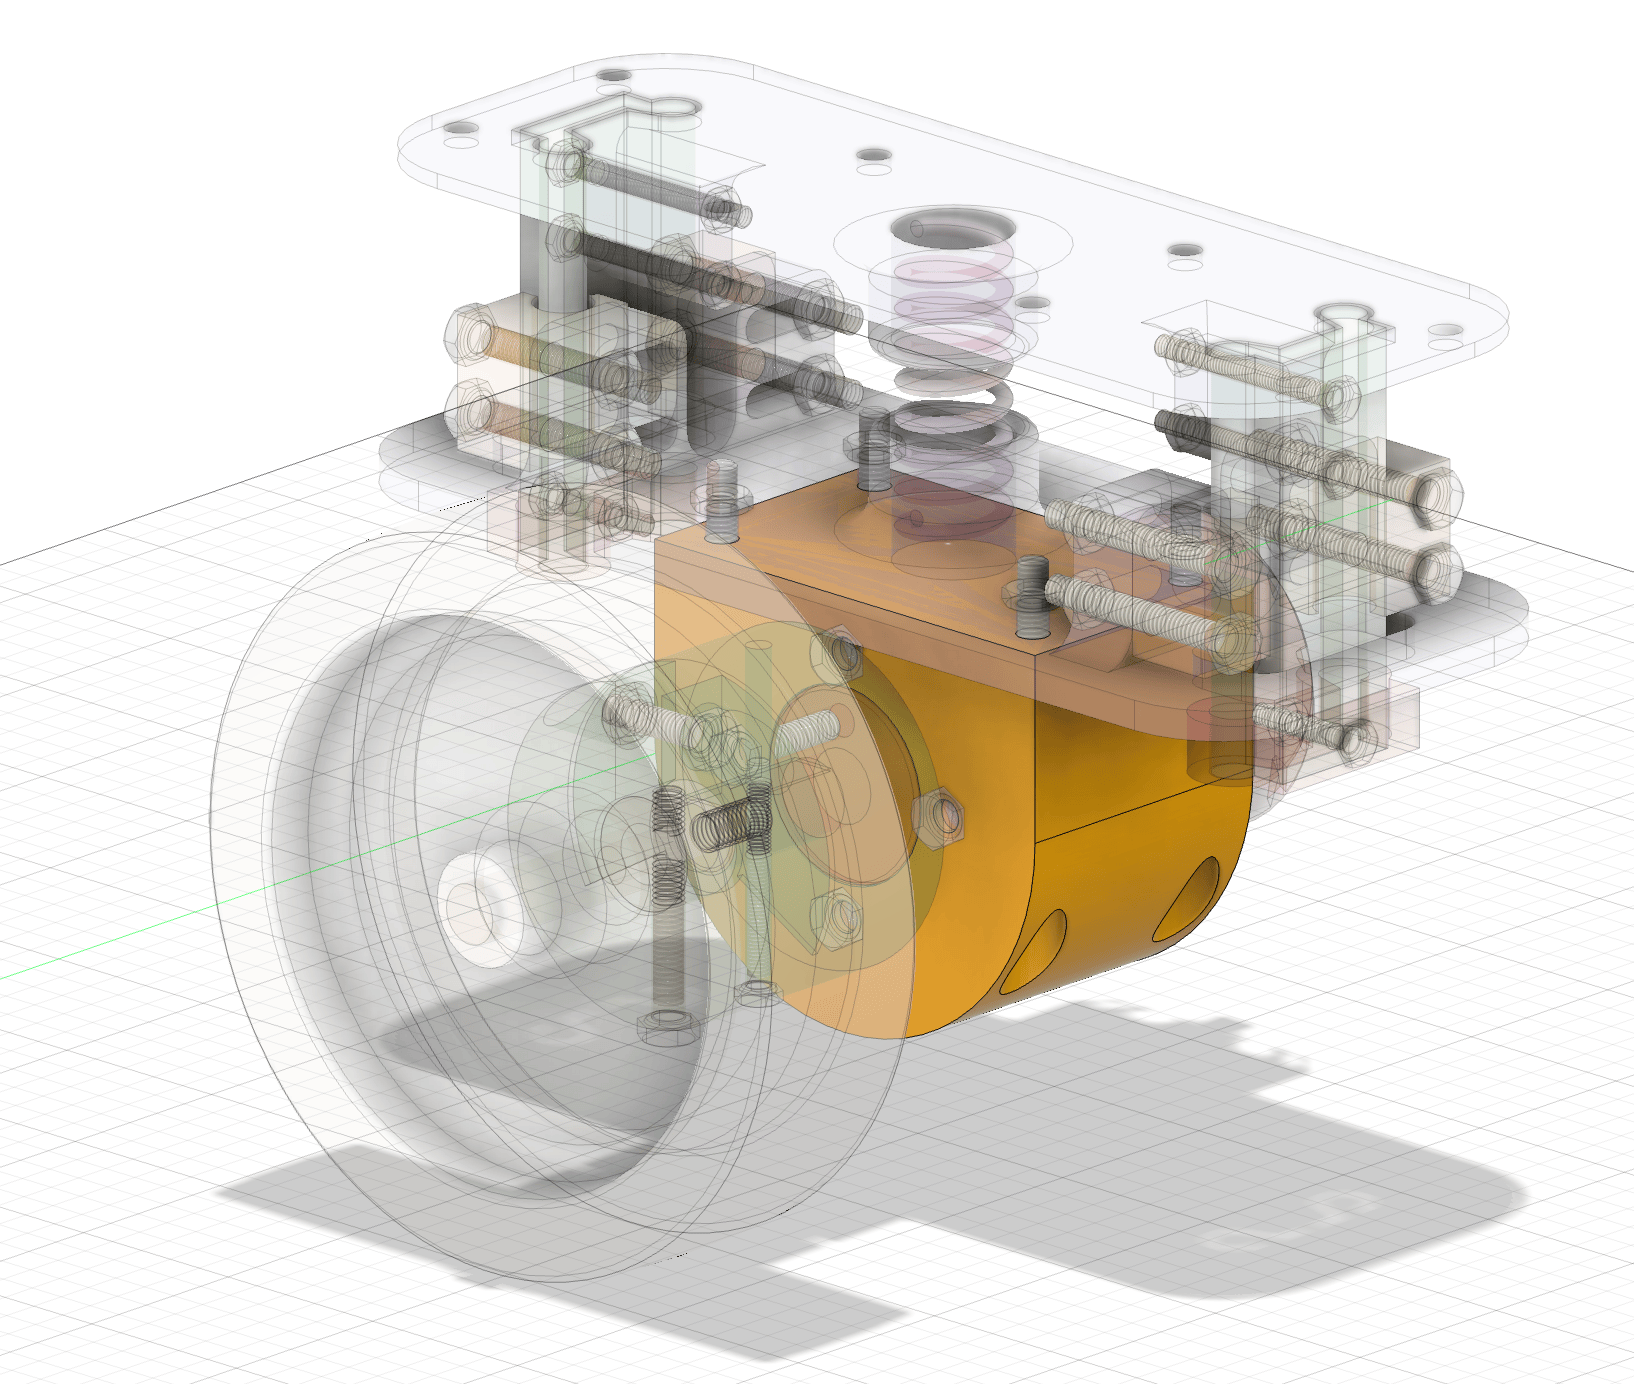
\includegraphics[width=\textwidth]{images/CAD design/Motor support.png}
        \end{minipage}
        &
        \begin{minipage}[t]{\linewidth}
        \vspace{0pt}
        \textbf{Motor support} \\ The motor support is designed to hold the motor in place and provide stability during operation ensuring it can withstand the forces generated by the motor and the suspension system.
        \end{minipage}
        \\
    \end{tabular}}
\end{table}

\begin{table}[H]
    \centering
    \resizebox{\textwidth}{!}{
    \begin{tabular}[t]{@{}m{0.4\textwidth} m{0.6\textwidth}@{}}
        \begin{minipage}[t]{\linewidth}
        \vspace{0pt}
        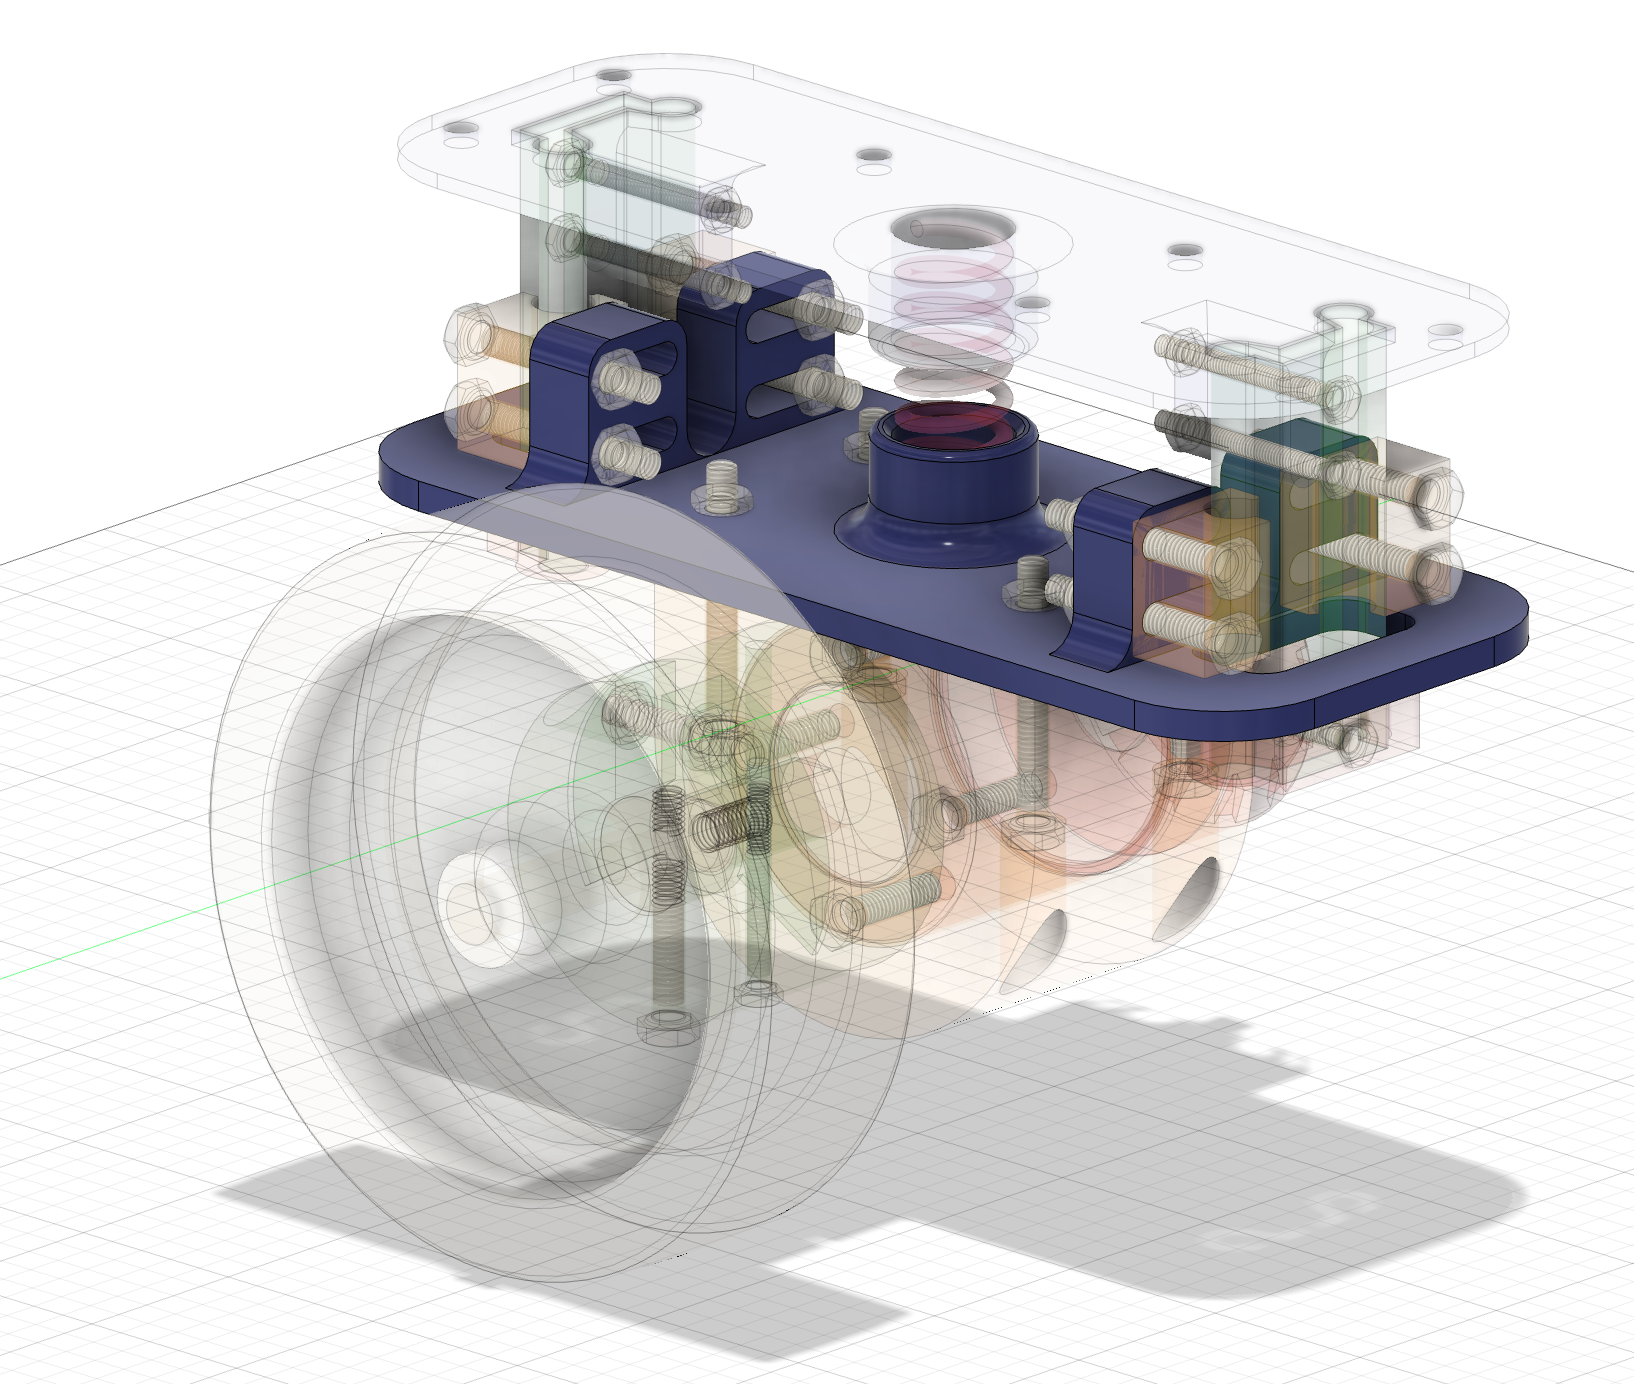
\includegraphics[width=\textwidth]{images/CAD design/Base motor support.png}
        \end{minipage}
        &
        \begin{minipage}[t]{\linewidth}
        \vspace{0pt}
        \textbf{Base motor support} \\ The base motor support is the foundation of the suspension system, providing a stable platform for the motor and other components. It has been designed to hold in place the guide sliders allowing the guide to pass through the holes in it. Furthermore, it has been designed a dovetail way in order to provide the correct alignment with the motor support.
        \end{minipage}
        \\
    \end{tabular}}
\end{table}

\begin{table}[H]
    \centering
    \resizebox{\textwidth}{!}{
    \begin{tabular}[t]{@{}m{0.4\textwidth} m{0.6\textwidth}@{}}
        \begin{minipage}[t]{\linewidth}
        \vspace{0pt}
        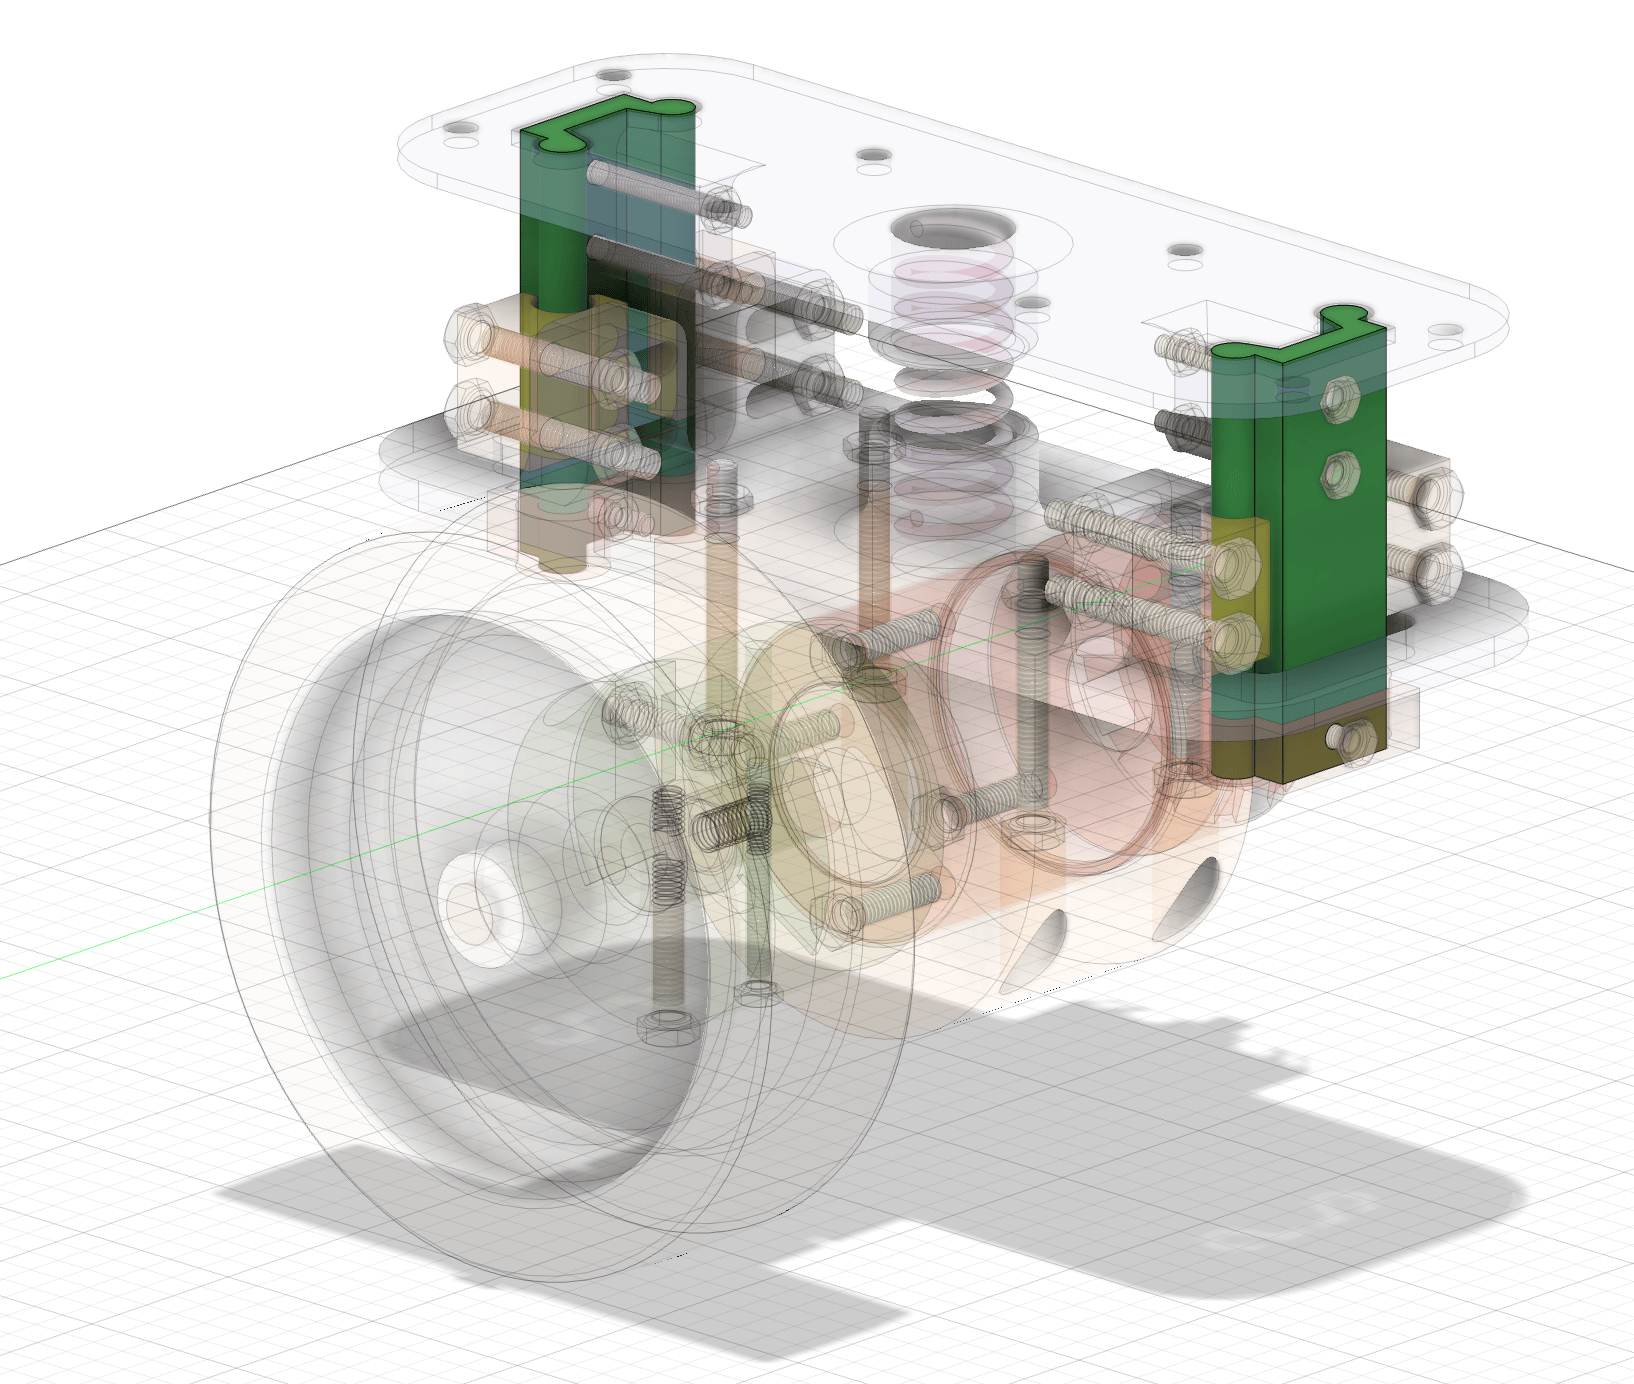
\includegraphics[width=\textwidth]{images/CAD design/Guide.png}
        \end{minipage}
        &
        \begin{minipage}[t]{\linewidth}
        \vspace{0pt}
        \textbf{Guide} \\ The guide is a component that helps to maintain the alignment of the suspension system, ensuring smooth and controlled movement. It is lightweight providing at the same time the necessary support without adding excessive weight to the overall system.
        \end{minipage}
        \\
    \end{tabular}}
\end{table}

\begin{table}[H]
    \centering
    \resizebox{\textwidth}{!}{
    \begin{tabular}[t]{@{}m{0.4\textwidth} m{0.6\textwidth}@{}}
        \begin{minipage}[t]{\linewidth}
        \vspace{0pt}
        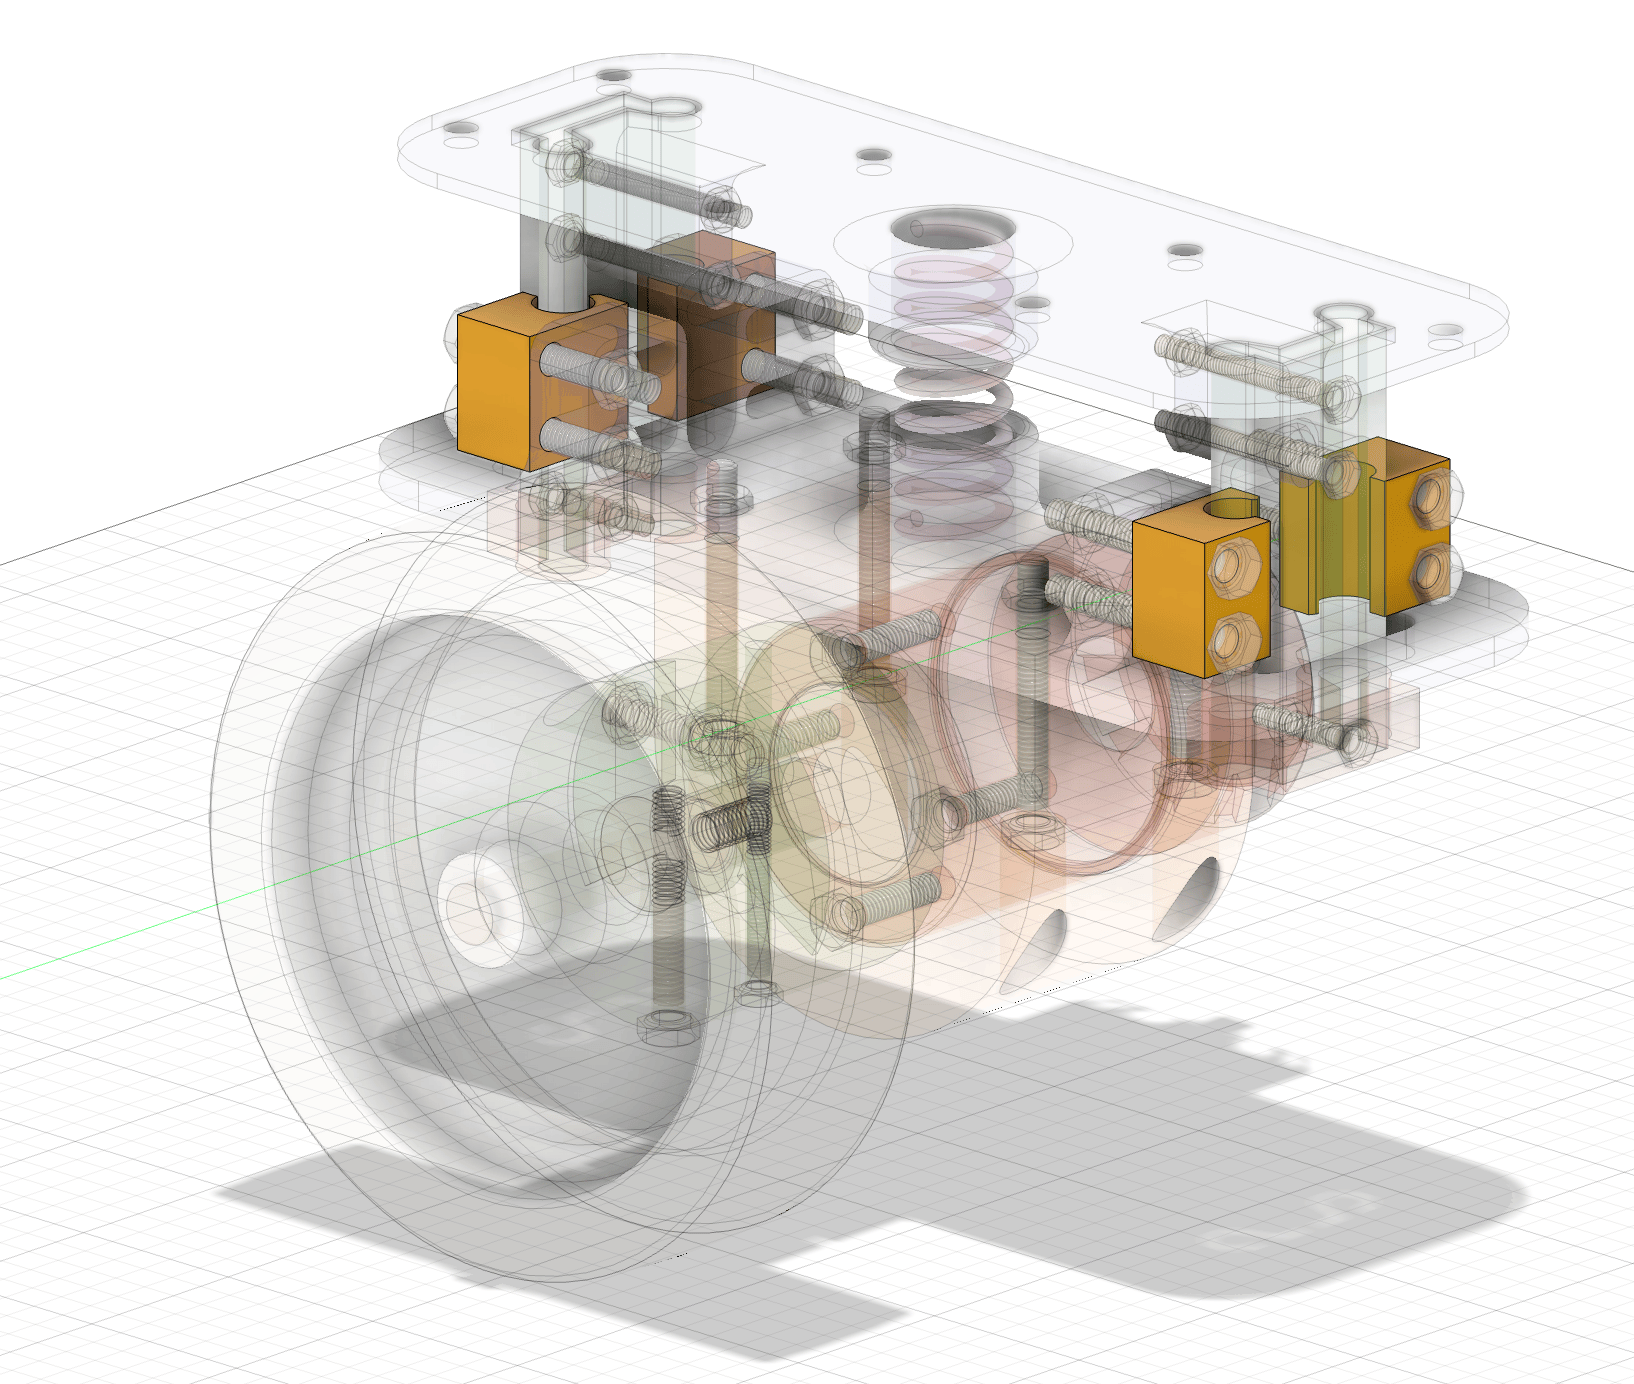
\includegraphics[width=\textwidth]{images/CAD design/Guide sliders.png}
        \end{minipage}
        &
        \begin{minipage}[t]{\linewidth}
        \vspace{0pt}
        \textbf{Guide sliders} \\ The guide sliders are the complementary components to the guide, allowing, as their name suggests, smooth sliding motion along the guide rails. They are designed to reduce friction and wear, ensuring long-lasting performance and reliability.
        \end{minipage}
        \\
    \end{tabular}}
\end{table}

\begin{table}[H]
    \centering
    \resizebox{\textwidth}{!}{
    \begin{tabular}[t]{@{}m{0.4\textwidth} m{0.6\textwidth}@{}}
        \begin{minipage}[t]{\linewidth}
        \vspace{0pt}
        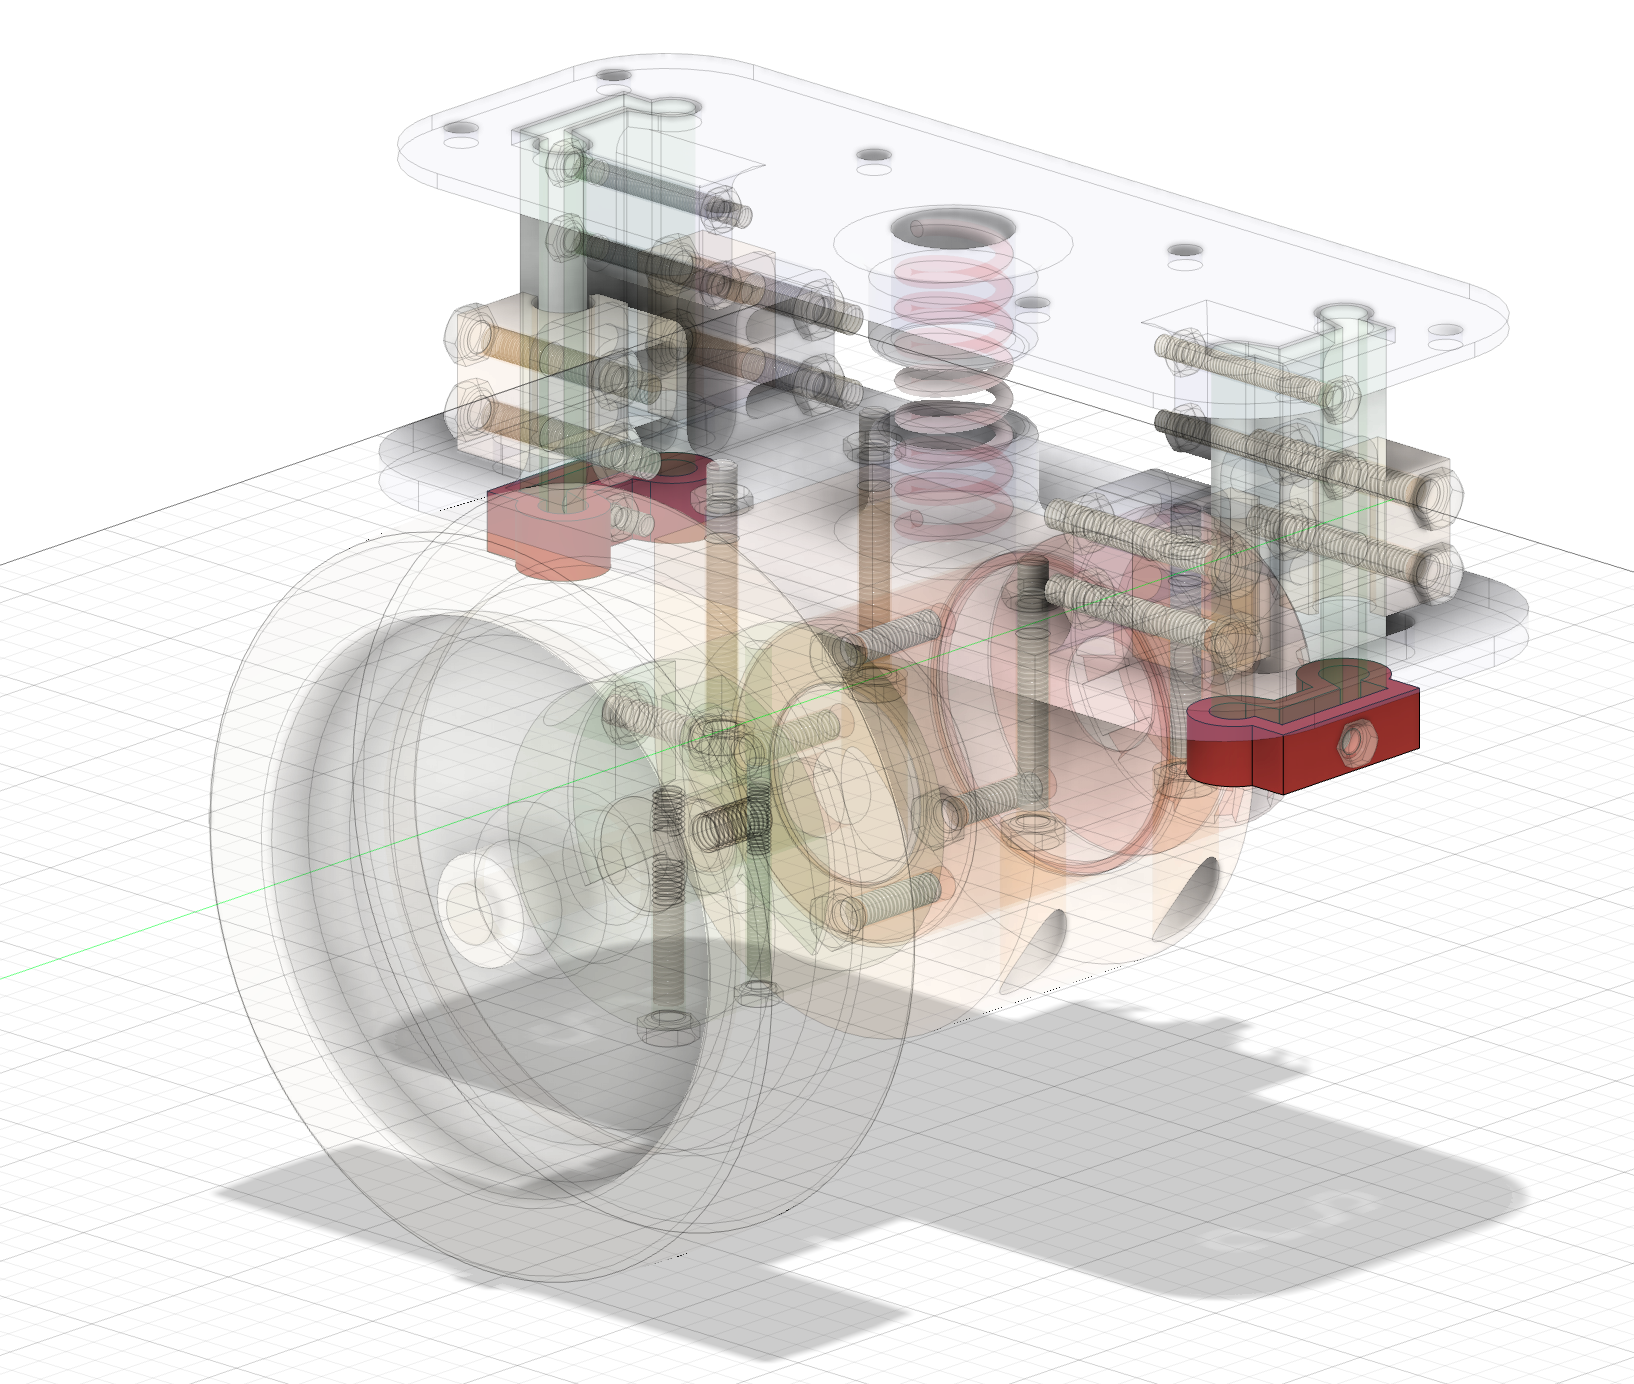
\includegraphics[width=\textwidth]{images/CAD design/Guide end stop.png}
        \end{minipage}
        &
        \begin{minipage}[t]{\linewidth}
        \vspace{0pt}
        \textbf{Guide end stop} \\ The guide end stop is a component that has been designed to lock the vertical movement of the spring in order to avoid the spring to come out as well as the bottom part of the suspension system.
        \end{minipage}
        \\
    \end{tabular}}
\end{table}

\begin{table}[H]
    \centering
    \resizebox{\textwidth}{!}{
    \begin{tabular}[t]{@{}m{0.4\textwidth} m{0.6\textwidth}@{}}
        \begin{minipage}[t]{\linewidth}
        \vspace{0pt}
        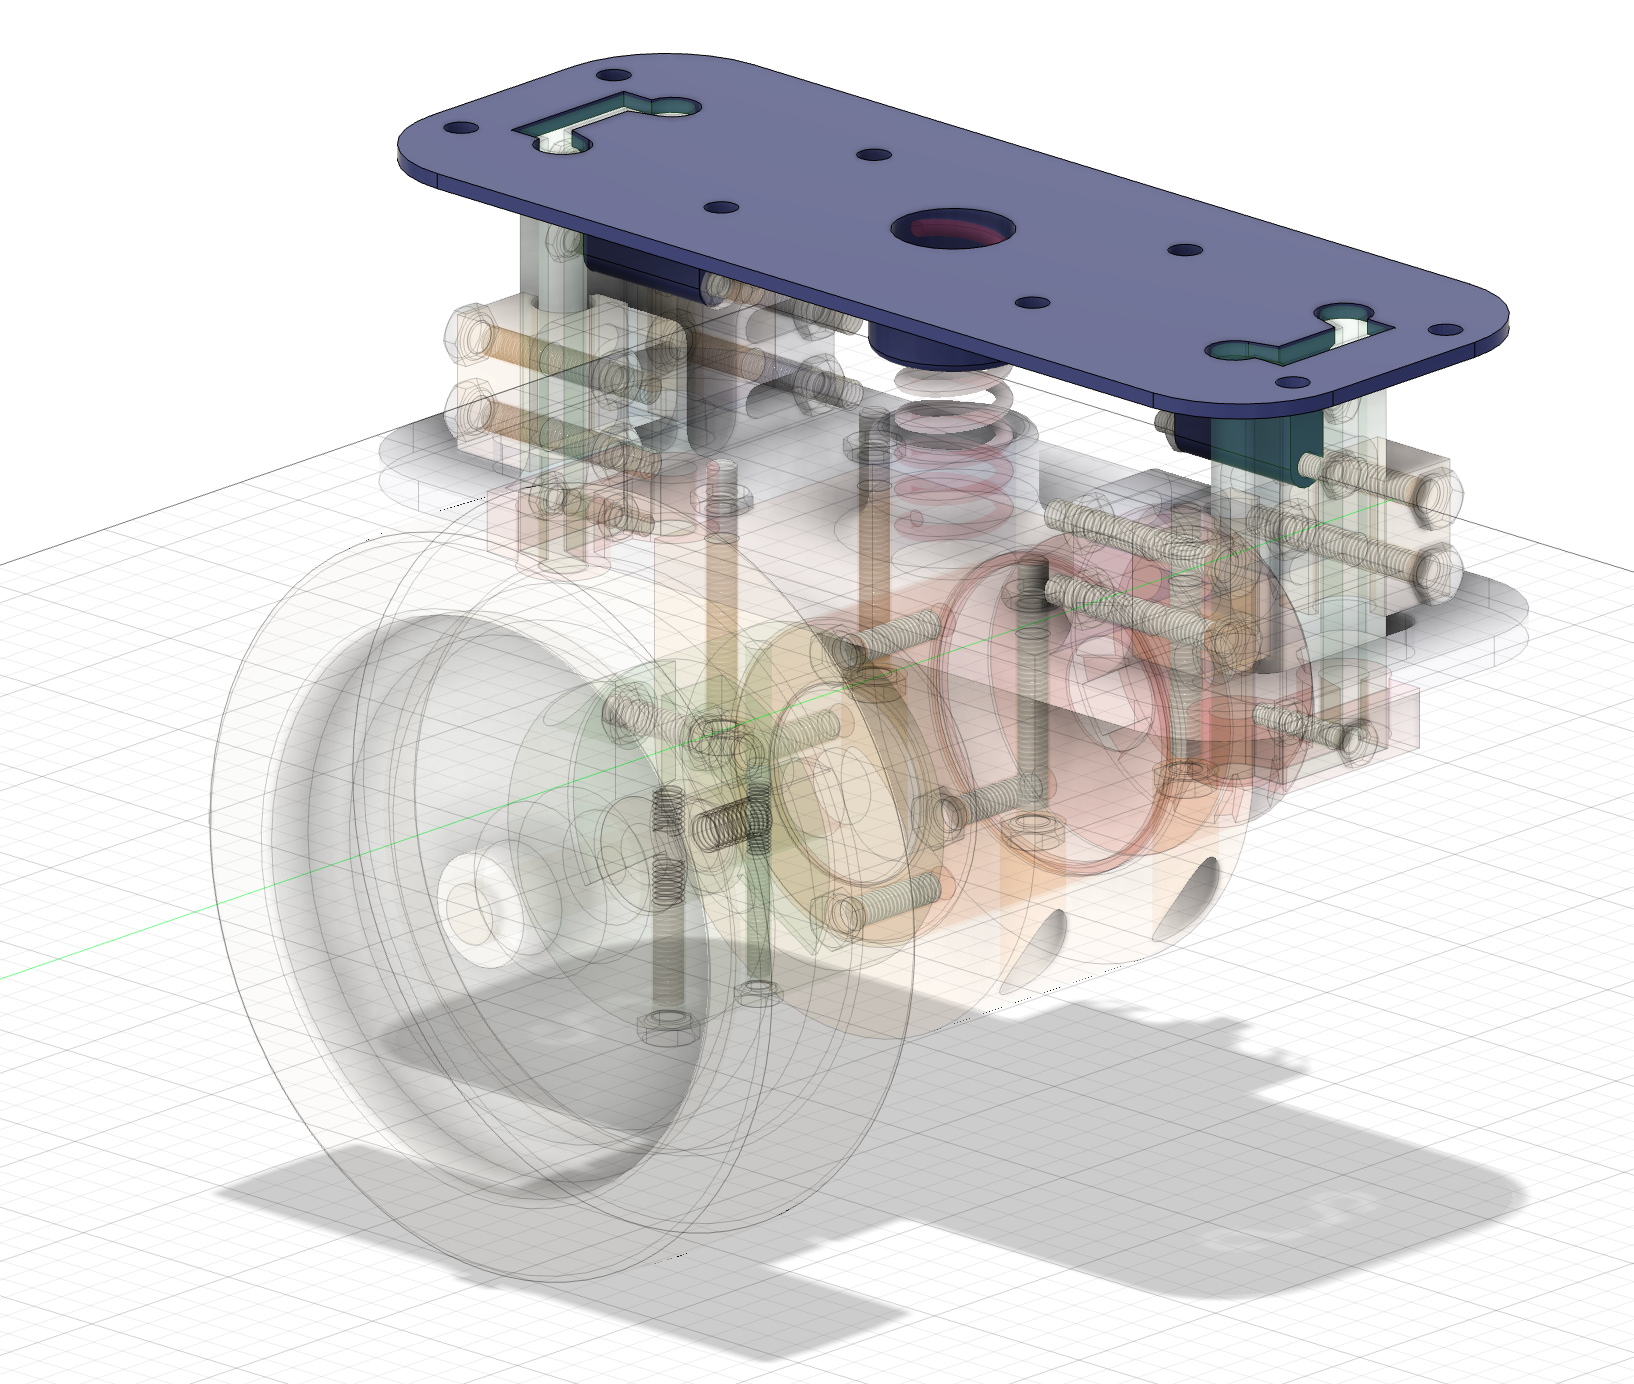
\includegraphics[width=\textwidth]{images/CAD design/Base platform.png}
        \end{minipage}
        &
        \begin{minipage}[t]{\linewidth}
        \vspace{0pt}
        \textbf{Base platform} \\ As well as the base motor support, the base platform is designed to provide a stable foundation for the entire suspension system. It is made from lightweight materials to minimize weight while maintaining strength and rigidity when linked to the platform.
        \end{minipage}
        \\
    \end{tabular}}
\end{table}


\begin{table}[H]
    \centering
    \resizebox{\textwidth}{!}{
    \begin{tabular}[t]{@{}m{0.4\textwidth} m{0.6\textwidth}@{}}
        \begin{minipage}[t]{\linewidth}
        \vspace{0pt}
        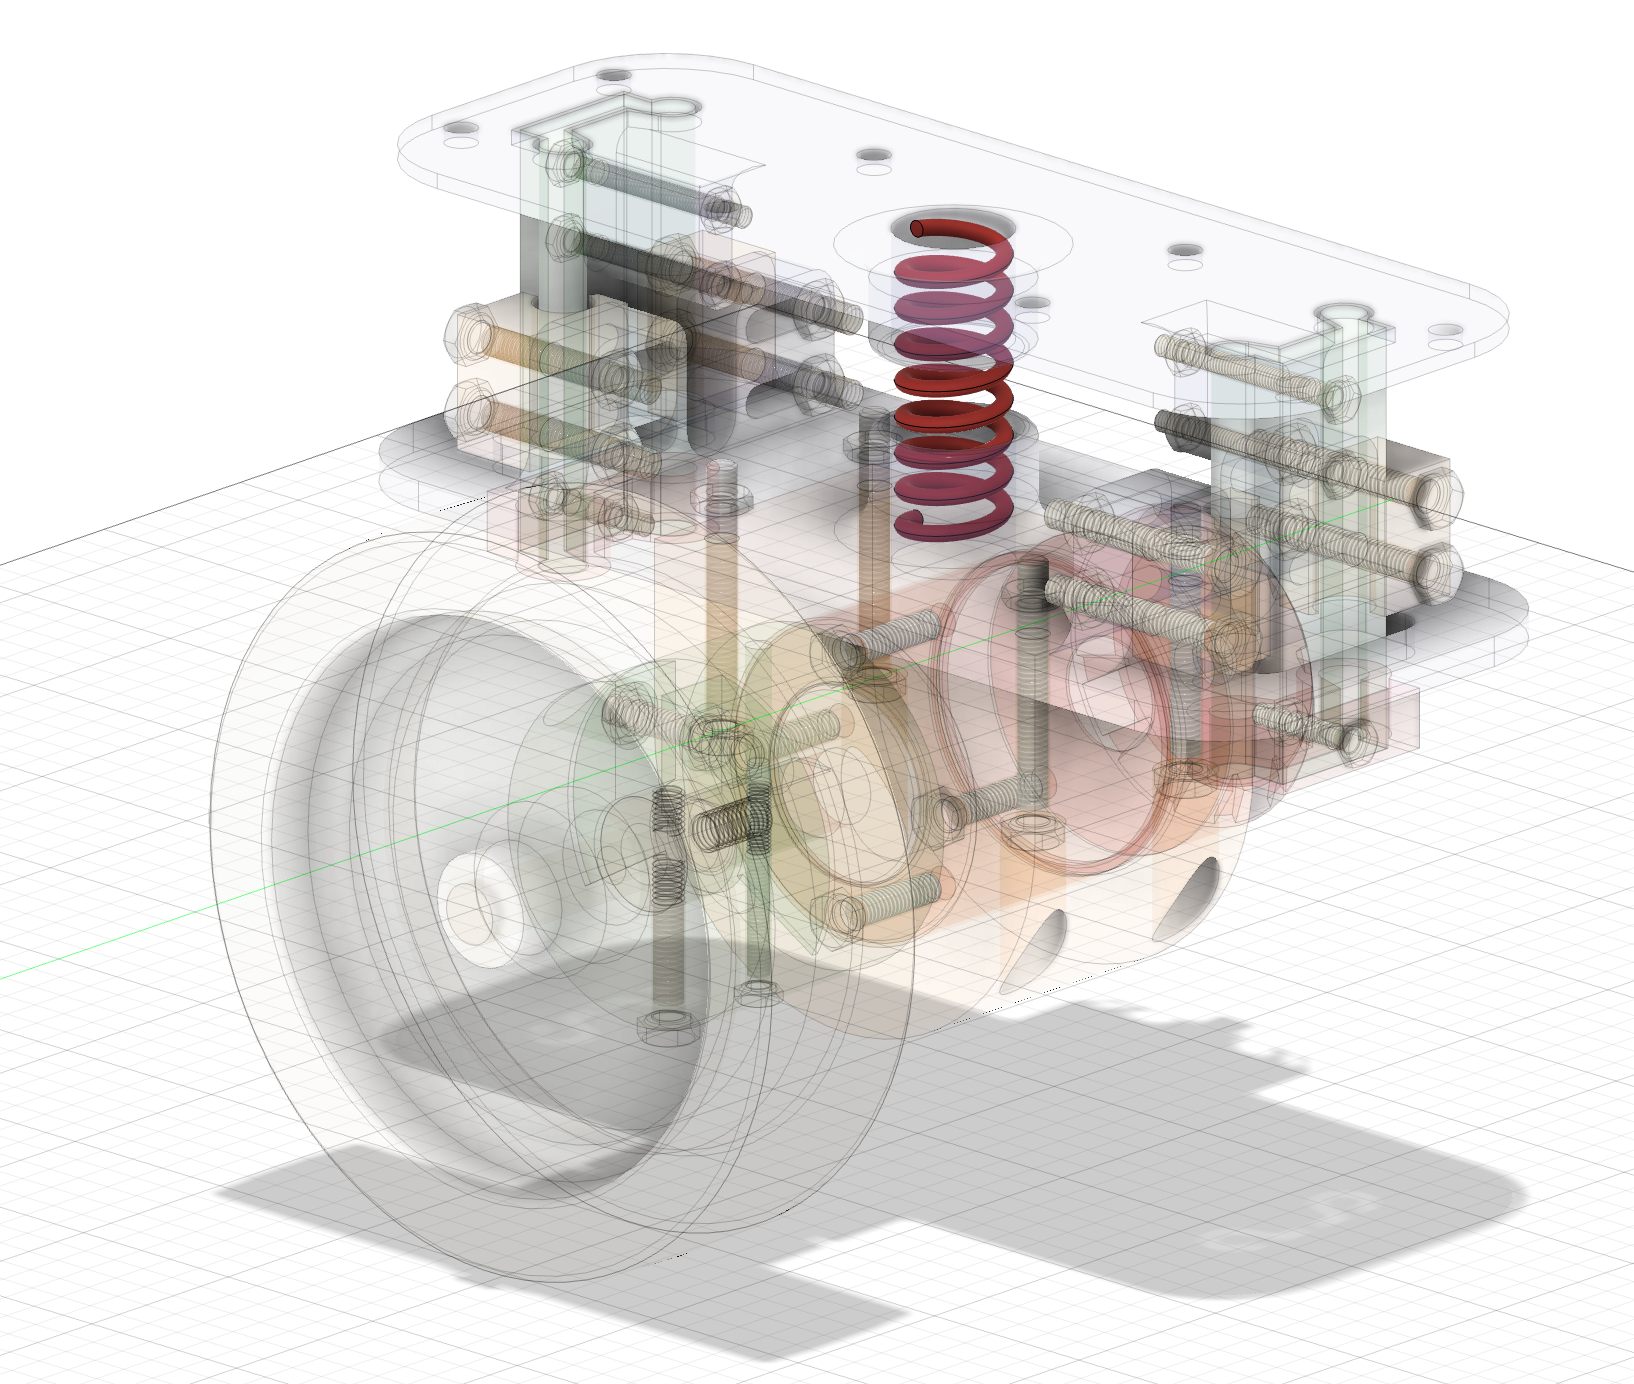
\includegraphics[width=\textwidth]{images/CAD design/Spring.png}
        \end{minipage}
        &
        \begin{minipage}[t]{\linewidth}
        \vspace{0pt}
        \textbf{Spring} \\ The spring is the core component of the suspension system, providing the necessary force to support the AMR's weight and absorb shocks from uneven terrain. The spring is designed to be adjustable in terms of length and stiffness, allowing for customization based on the AMR's payload and operating conditions.
        \end{minipage}
        \\
    \end{tabular}}
\end{table}

\newpage

\section{Analysis}
\subsection{Material Selection}
Firstly, before proceeding with the analysis, it is important to highlight the material selection process. The material used for the suspension system affects different parameters used in the following analysis. As a matter of fact, values for the parameters have been found in the literature based on the spring material of each spring found, as shown in the Table \ref{tab:spring_parametric_design}:

\begin{table}[H]
    \centering
    \resizebox{\textwidth}{!}{
    \begin{tabular}{|c|c|c|c|c|c|c|}
    \rowcolor{blue!5}
        \hline
        \textbf{Material} & \textbf{$R_m$ [MPa]} & \textbf{$R_{eh}$ [MPa]} & \textbf{$G$ [GPa]} & \textbf{$b_D$ [/]} & \textbf{$\Delta \tau_0$ [MPa]} & \textbf{$b_\tau$ [/]} \\
        \hline
        Filo di acciaio armonico & 2100 & 1785 & 81000 & 1.0 & 450 & 0.3 \\
        Acciaio inossidabile 302 & 1700 & 1275 & 74000 & 1.0 & 300 & 0.3 \\
        Acciaio inossidabile 316 & 1350 & 1050 & 73000 & 1.0 & 270 & 0.3 \\
        Acciaio zincato & 2100 & 1785 & 81000 & 1.0 & 450 & 0.3 \\
        \hline
    \end{tabular}}
    \caption{Material properties used in the analysis}
    \label{tab:material_properties}
\end{table}

\noindent
Delving into the Table \ref{tab:material_properties}, it is possible to highlight the meaning of each parameter:
\begin{itemize}
    \item \textbf{Ultimate tensile strength (\( R_m \))} \\ The maximum stress that a material can withstand while being stretched or pulled before necking.
    \item \textbf{Yield strength (\( R_{eh} \))} \\ The stress at which a material begins to deform plastically.
    \item \textbf{Shear modulus (\( G \))} \\ A measure of the material's ability to deform under shear stress.
    \item \textbf{Diameter factor (\( b_D \))} \\ A correction factor that accounts for the effect of the spring's diameter on its performance.
    \item \textbf{Torsional fatigue strength (\( \Delta \tau_0 \))} \\ The maximum shear stress that a material can withstand for a specified number of cycles without failure.
    \item \textbf{Mean stress penalty factor (\( b_\tau \))} \\ A factor that accounts for the effect of mean stress on the material's fatigue strength.
\end{itemize}

\newpage

\subsection{Static Load Analysis}
The static load analysis is a crucial step in the design process, ensuring that the suspension system can withstand the forces generated during operation. The purpose of this analysis is to determine a safety factor for the spring, ensuring that it can support the maximum payload without failure.

It is important to highlight that the payload is distributed evenly across the four non-driven wheels of the platform and the two driven wheels. Because of that, a force distribution percentage has been involved in the calculus of the static load analysis. 

\vskip1em
\noindent
It is possible to calculate the static load safety factor as follows:
\begin{equation}
    \text{CS}_\text{sta} = \frac{\tau_\text{amm}}{\tau_\text{max}} \ge 1
\end{equation}
where:
\begin{itemize}
    \item \( \tau_\text{amm} \) is the maximum allowable shear stress for the material used in the spring.
    \item \( \tau_\text{max} \) is the maximum shear stress applied to the spring.
\end{itemize}

\vskip4em
\subsubsection{Admissible Stress}
The admissible stress is calculated using the following equation since the spring has been subjected to cold working processes:
\begin{equation}
    \tau_\text{amm} = 0.5 \cdot R_m
\end{equation}

\noindent
where:
\begin{itemize}
    \item \( R_m \) is the ultimate tensile strength of the material used in the spring (refer to Table \ref{tab:material_properties}).
\end{itemize}

\newpage
\subsubsection{Maximum Stress}
The maximum stress applied to the spring is calculated using the following equation:
\begin{equation}
    \tau_\text{max} = \lambda' \cdot \frac{8 \cdot F_\text{eff} \cdot c}{\pi \cdot d^2}
\end{equation}
where:
\begin{itemize}
    \item $\lambda'$ is first Wahl's correction factor
    \item \( F_\text{eff} \) is the effective force on the spring (parametric due to the payload).
    \item $c$ is the spring index
    \item $d$ is the wire diameter of the spring
\end{itemize}

\noindent
Delving even deeper into the equation, it is possible to define the calculus of each parameter:
\begin{align}
    & c = \frac{D}{d} \\[1em]
    & \lambda' = \frac{4c -1}{4c - 4} + \frac{0.615}{c} \\[1em]
    & F_\text{eff} = \frac{k_\text{dist} \cdot m \cdot g}{N_\text{wheels}}
\end{align}
where:
\begin{itemize}
    \item \( k_\text{dist} = 0.2\) \\ distribution factor, accounting for the non-uniform load distribution among the wheels.
    \item \( m = \text{parametric}\) \\ total mass of the AMR (payload + empty weight).
    \item \( g = 9.80665 \,m/s^2\) \\ gravitational acceleration.
    \item \( N_\text{wheels} = 4\) \\ number of wheels in contact with the ground.
\end{itemize}
\newpage

\subsection{Fatigue Analysis}
As well as the static load analysis, the fatigue analysis is a pivotal step in the design process, ensuring that the suspension system can withstand repeated loading and unloading cycles without failure. The purpose of this analysis is to determine a safety factor for the spring, ensuring that it can support the maximum payload over a specified number of cycles.

\vskip1em
It is possible to calculate the fatigue safety factor as follows:
\begin{equation}
    \text{CS}_\text{fat} = \frac{\Delta \tau_\text{amm}}{\Delta \tau_\text{max}} \ge 1
\end{equation}
where:
\begin{itemize}
    \item \( \Delta \tau_\text{amm} \) is the maximum allowable shear stress for the material used in the spring.
    \item \( \Delta \tau_\text{max} \) is the maximum shear stress applied to the spring.
\end{itemize}

\vskip4em
\subsubsection{Admissible Stress}
In a similar way to the static load analysis, the admissible stress is calculated using the following equation:
\begin{equation}
    \Delta \tau_\text{amm} = b_D \cdot \Delta \tau_0 - \beta_\tau \cdot \tau_ \text{min}
\end{equation}
where:
\begin{itemize}
    \item \( b_D \) is the diameter factor (refer to Table \ref{tab:material_properties}).
    \item \( \Delta \tau_0 \) is the torsional fatigue strength of the material used in the spring (refer to Table \ref{tab:material_properties}).
    \item \( \beta_\tau \) is a mean stress penalty factor (refer to Table \ref{tab:material_properties}).
    \item \( \tau_ \text{min}\) is the minimum shear stress applied to the spring.
\end{itemize}

\vskip1em
One more step is needed to calculate the admissible stress, which is the calculation of the minimum shear stress through the following equation:
\begin{equation}
    \tau_ \text{min} = \lambda''' \cdot \frac{8 \cdot F_\text{min} \cdot c}{\pi \cdot d^2}
\end{equation}
where:
\begin{itemize}
    \item \( \lambda''' \) is third Wahl's correction factor calculated as: $$\lambda''' = 1 + \frac{2}{c}$$
    \item \( F_\text{min} \) is the minimum force on the spring (parametric due to the payload).
    \item \( c \) is the spring index.
    \item \( d \) is the wire diameter of the spring.
\end{itemize}

\newpage
\subsubsection{Maximum Stress}
The maximum stress applied to the spring is calculated using the following equation:
\begin{equation}
    \Delta \tau_\text{max} = \lambda' \cdot \frac{8 \cdot \Delta F \cdot c}{\pi \cdot d^2}
\end{equation}
where:
\begin{itemize}
    \item \( \lambda' \) is first Wahl's correction factor.
    \item \( \Delta F \) is the force variation on the spring calculated as: $$\Delta F = F_\text{max} - F_\text{min}$$
    \item $c$ is the spring index.
    \item $d$ is the wire diameter of the spring.
\end{itemize}
\newpage

\subsection{FEM Simulations and ZEBRA Analysis}
The Finite Element Method (FEM) simulations were performed using Fusion360 (ANSYS environment) to validate the design and ensure that the suspension system meets the required
performance criteria. The simulations focused primarily on the static load, allowing for a detailed understanding of the stress distribution and deformation under various loading conditions.
On the other hand, the ZEBRA analysis was conducted to evaluate the surface continuity and smoothness of the suspension system's components. This analysis is crucial for ensuring that the suspension system can operate smoothly and efficiently.

The Finite Element Method (FEM) simulations were carried out using Fusion360, which provides the ANSYS simulation environment to validate the mechanical design and be sure that the suspension system meets the necessary structural and performance criteria. These simulations were instrumental in assessing how the system behaves under operational conditions. The analysis focused primarily on static load scenarios, providing valuable insight into the distribution of internal stresses and the deformation patterns that emerge when the suspension is subjected to different payload conditions. By examining these factors, it was possible to identify potential mechanical failures, optimize material usage, and ensure all components remain within their elastic limits.

In parallel, a ZEBRA analysis was performed to evaluate the surface continuity and smoothness of the suspension's components since they are essential not only for visual appeal but also for minimizing friction. The ZEBRA analysis helped identify any discontinuities, abrupt curvature changes, or imperfections in the surface geometry, allowing for refinements and enhancement.

Together, these simulation techniques played a key role in refining the suspension system design, ensuring structural integrity and optimal functionality.

\begin{figure}[H]
    \centering
    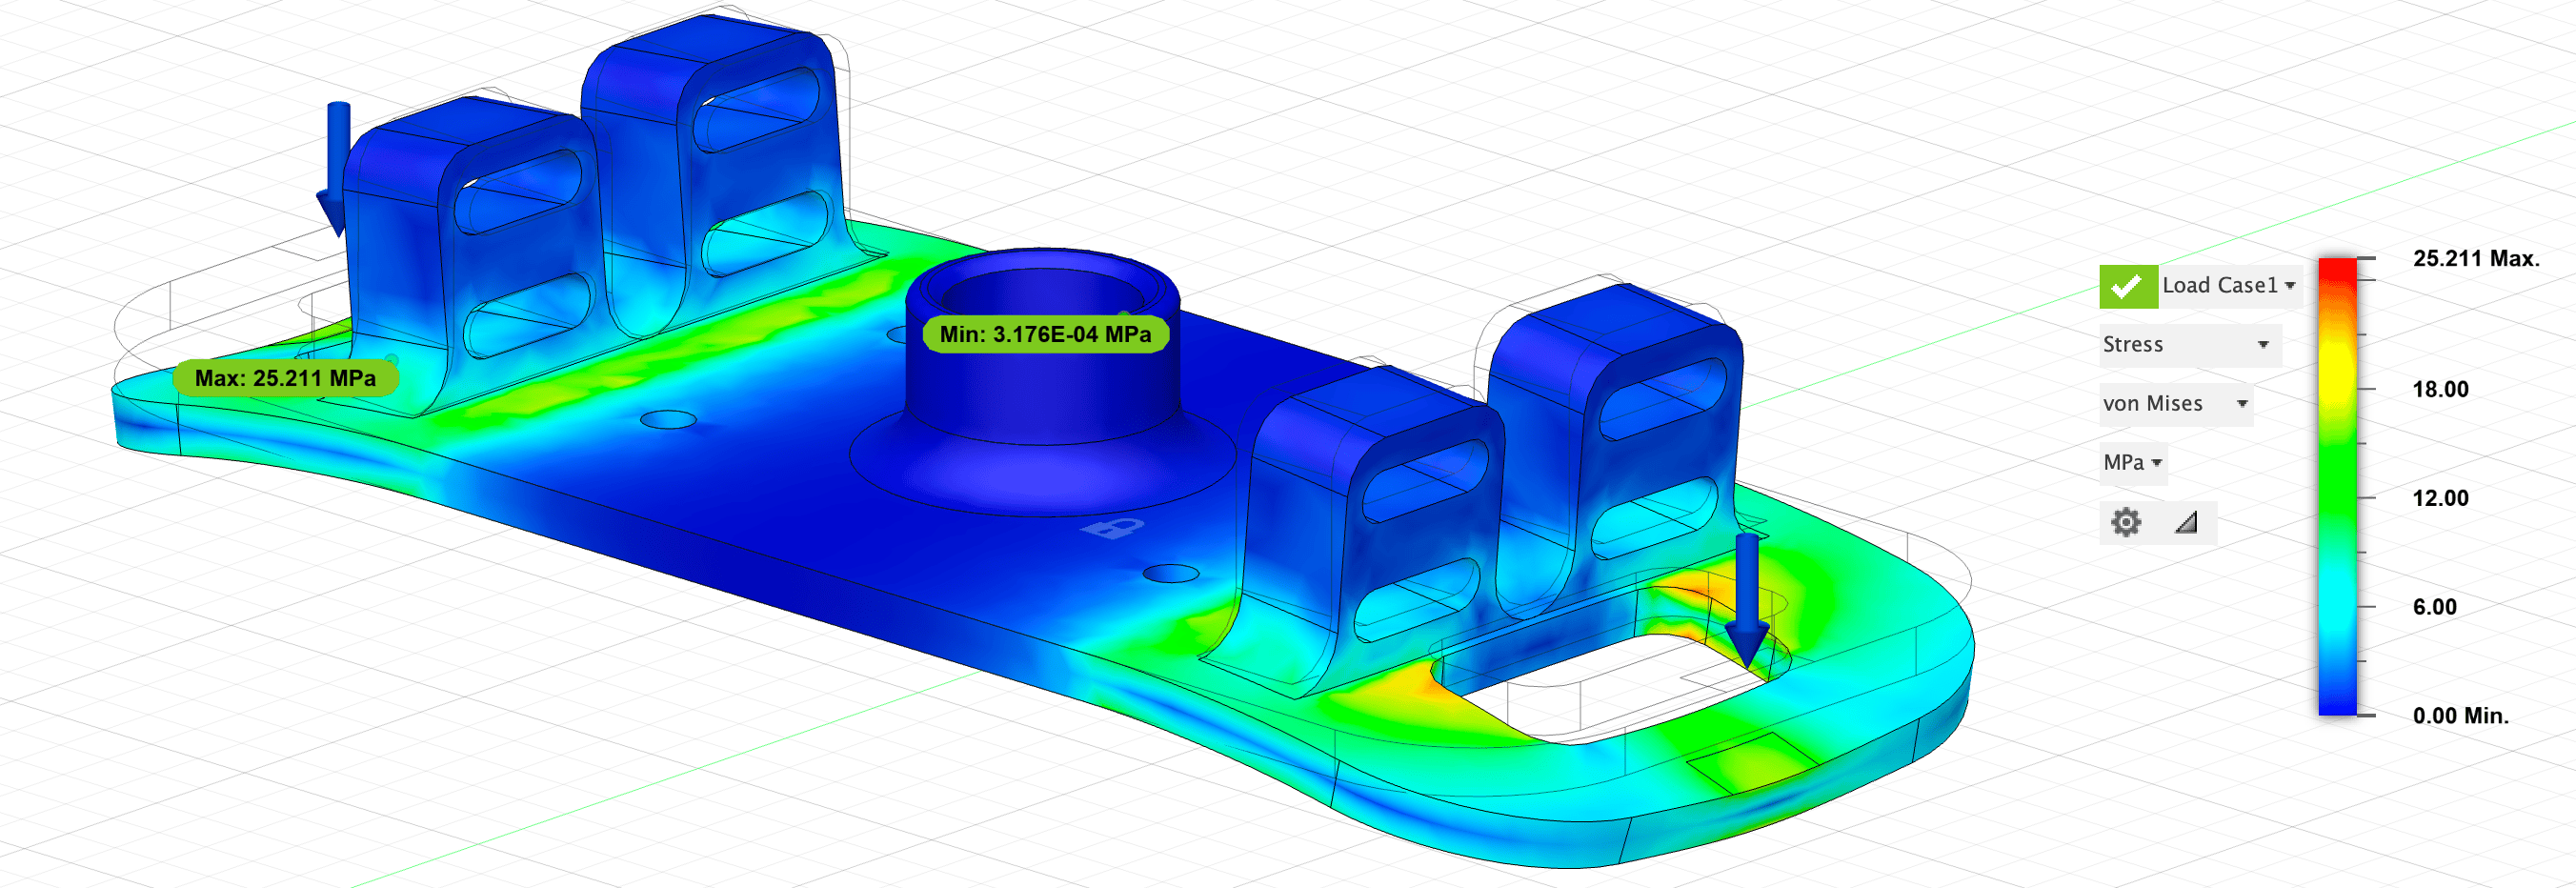
\includegraphics[width=0.9\textwidth]{images/FEM/baseMotorSupport.png}
    \caption{FEM simulation of the base motor support}
    \label{fig:fem_base_motor_support}
\end{figure}

\begin{figure}[H]
    \centering
    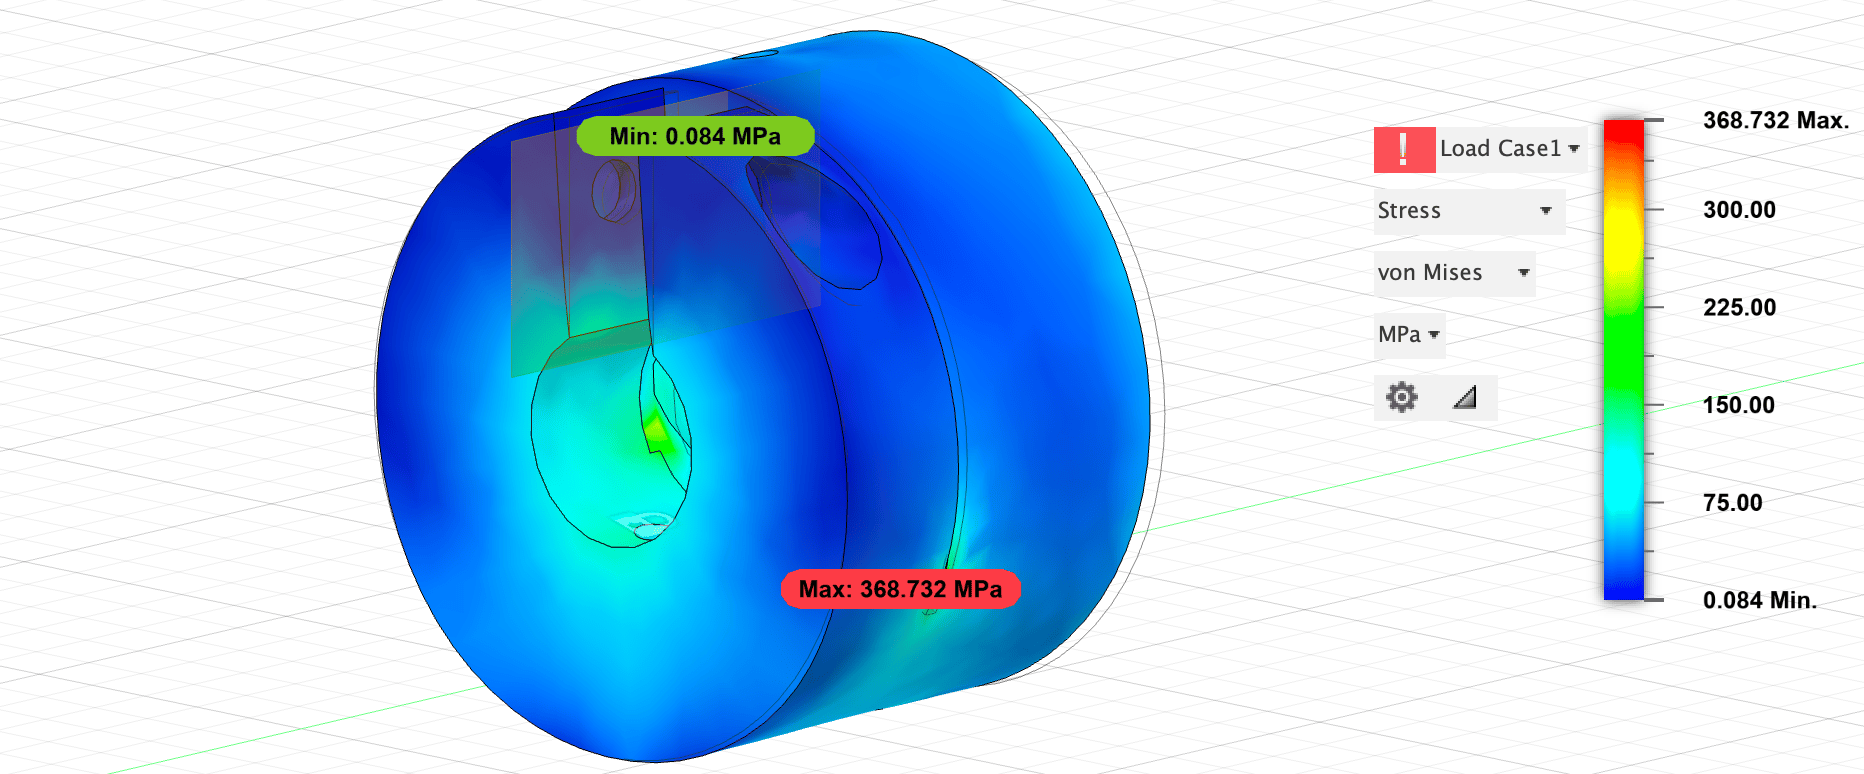
\includegraphics[width=0.9\textwidth]{images/FEM/adaptor.png}
    \caption{FEM simulation of the adaptor wheel-motor}
    \label{fig:fem_adaptor_wheel_motor}
\end{figure}

\begin{figure}[H]
    \centering
    \begin{minipage}{0.45\textwidth}
        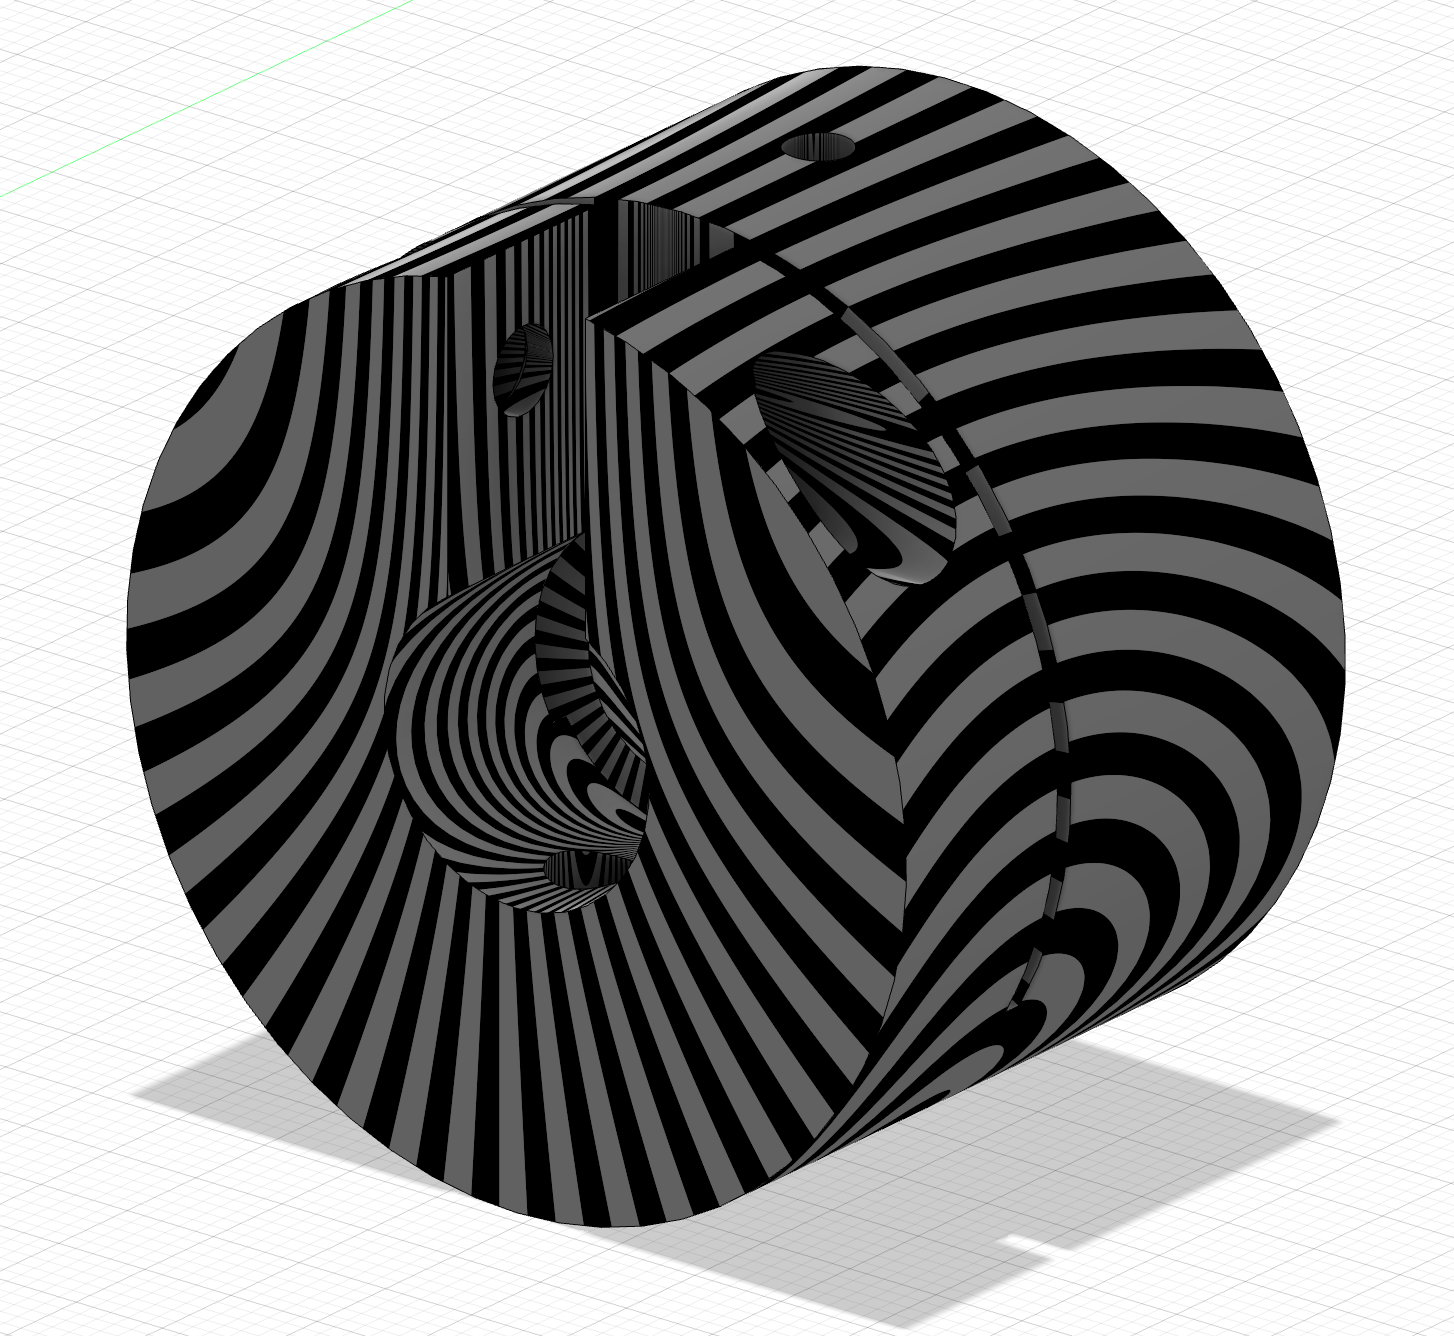
\includegraphics[width=\textwidth]{images/ZEBRA/adaptor1.png}
        \label{fig:zebra_adaptor_wheel_motor}
    \end{minipage}
    \hfill
    \begin{minipage}{0.45\textwidth}
        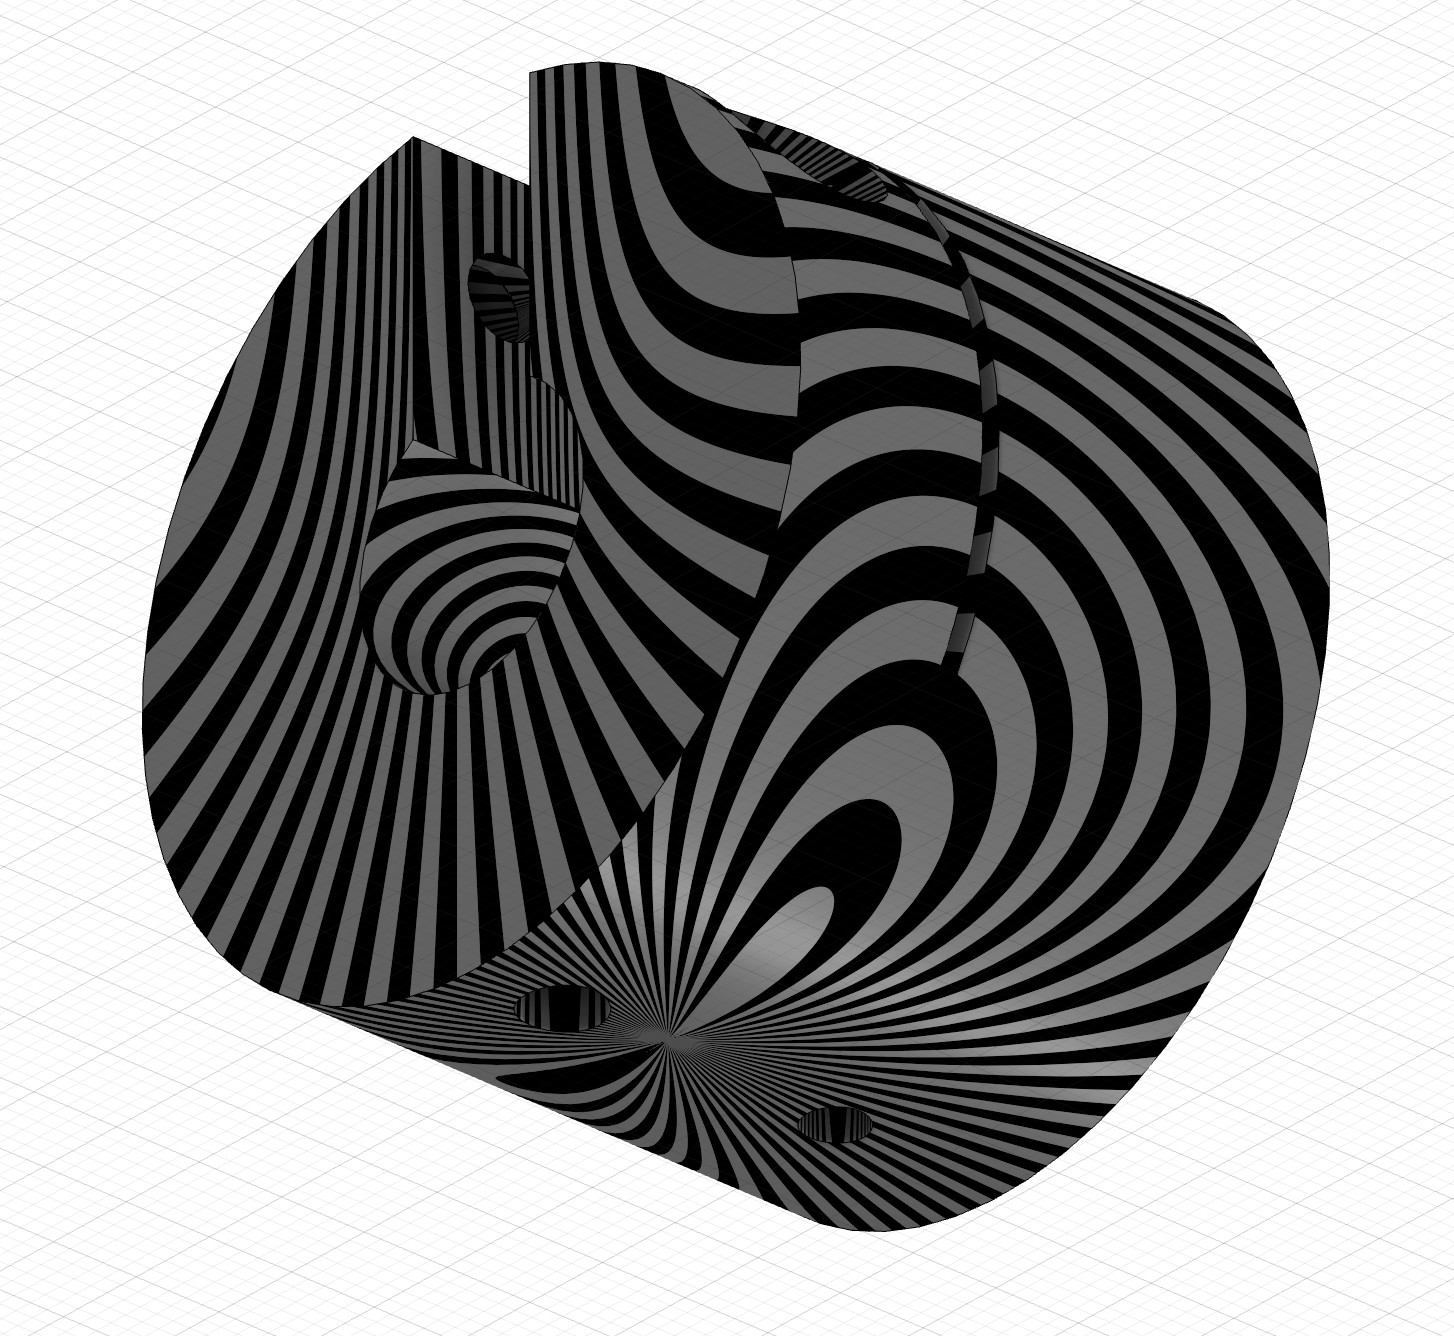
\includegraphics[width=\textwidth]{images/ZEBRA/adaptor2.png}
        \label{fig:zebra_adaptor_wheel_motor2}
    \end{minipage}
    \caption{ZEBRA analysis of the adaptor wheel-motor}
\end{figure}

\begin{figure}[H]
    \centering
    \begin{minipage}{0.45\textwidth}
        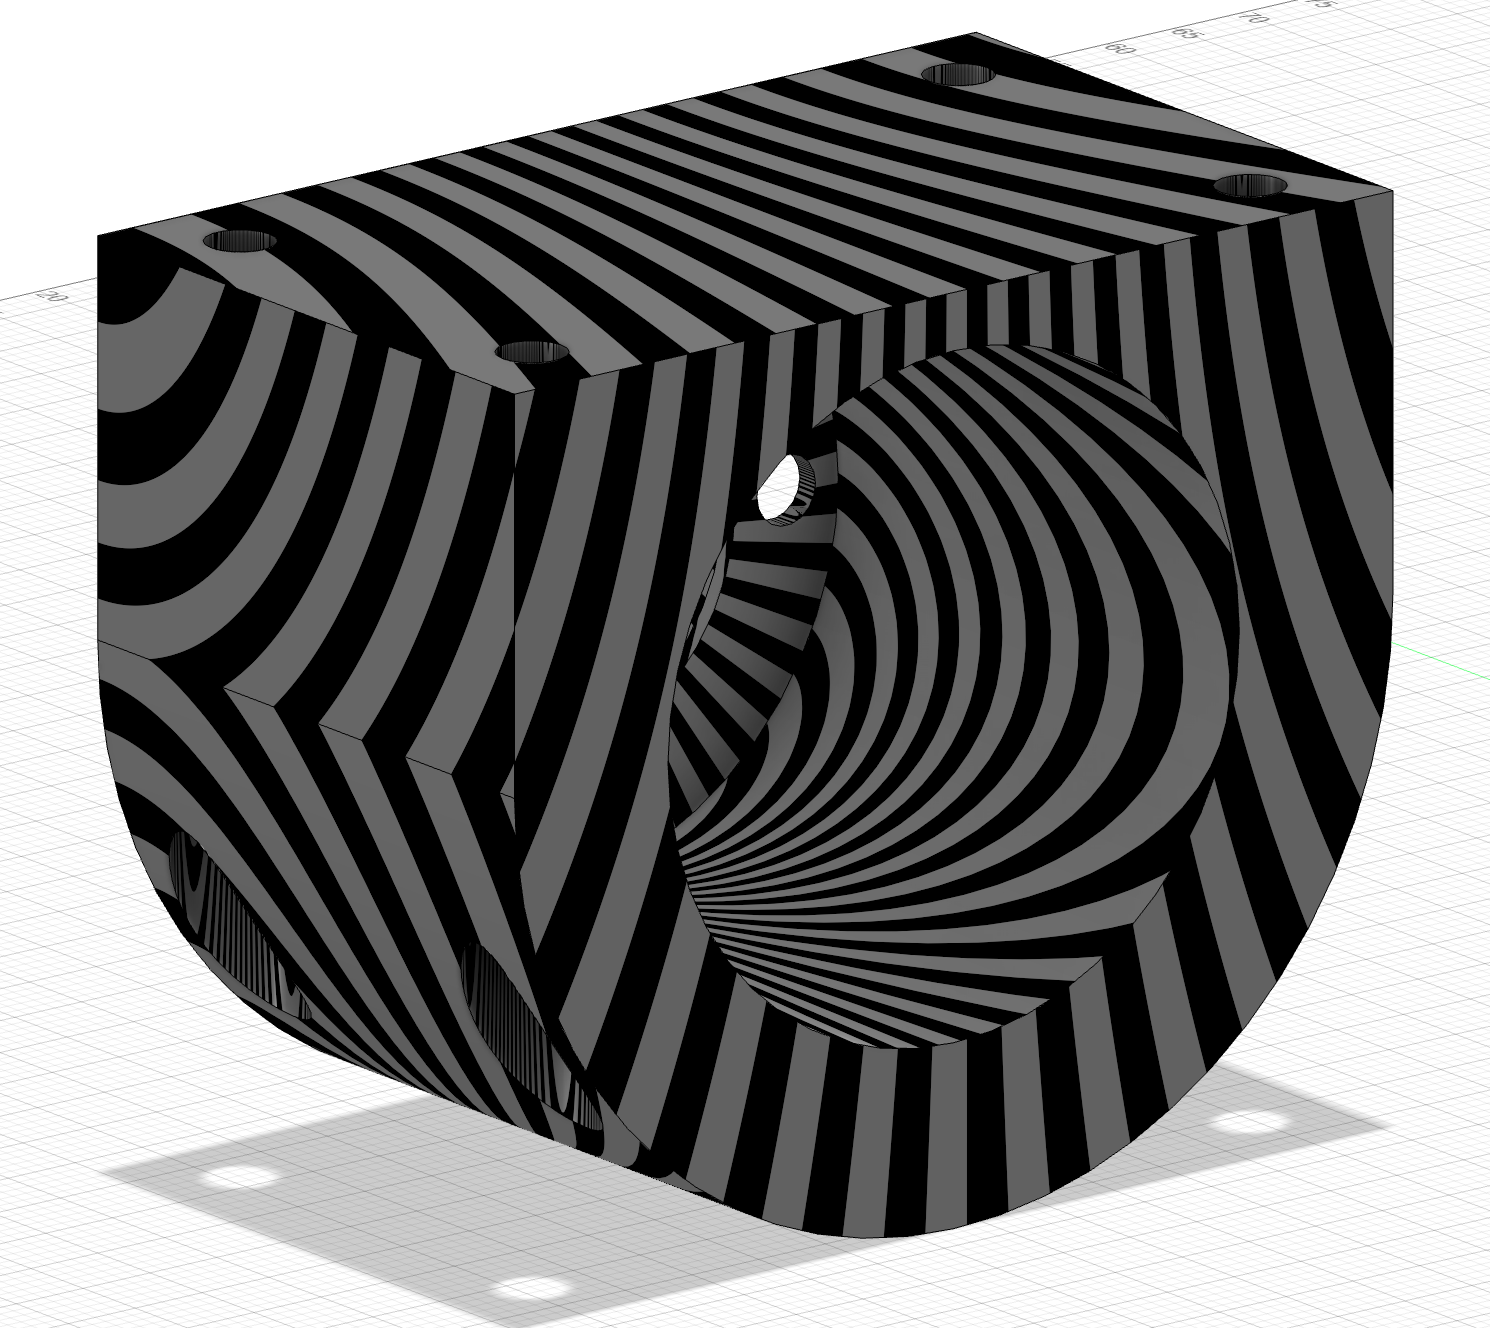
\includegraphics[width=\textwidth]{images/ZEBRA/motorSupport1.png}
        \label{fig:zebra_motor_support}
    \end{minipage}
    \hfill
    \begin{minipage}{0.45\textwidth}
        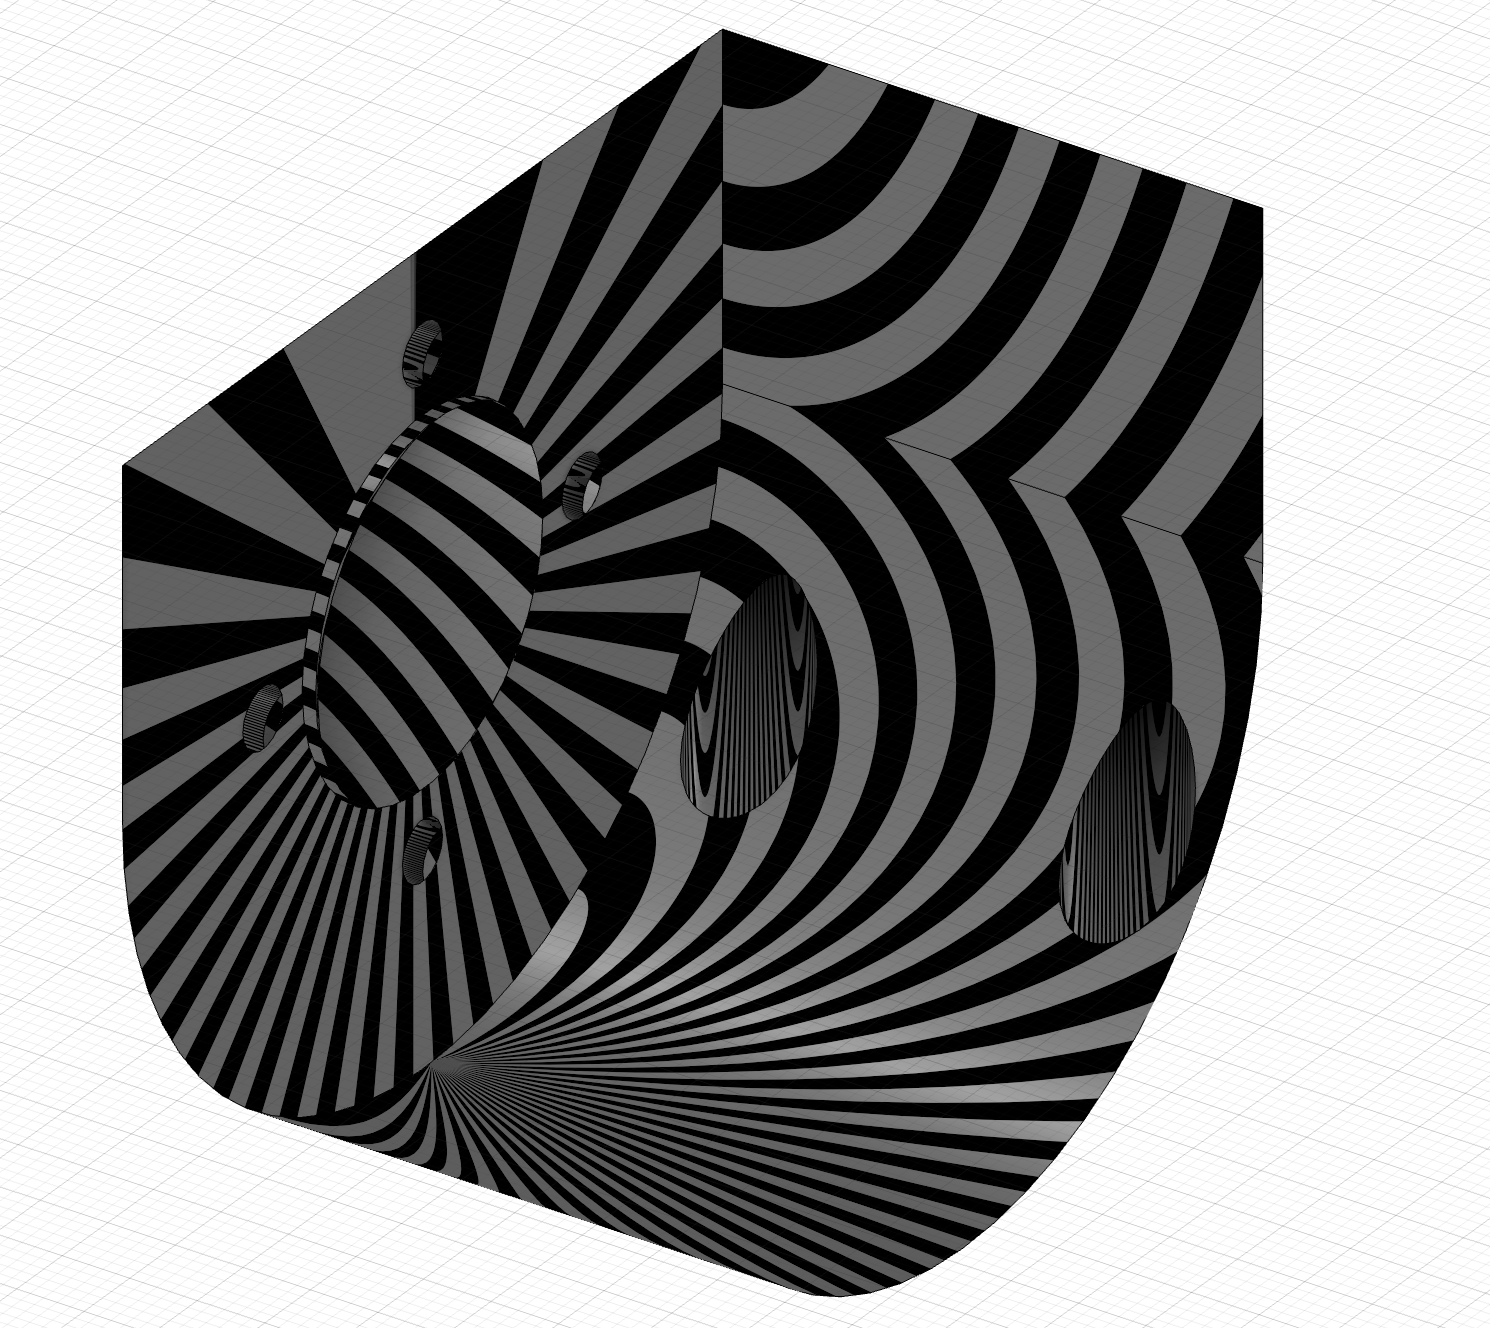
\includegraphics[width=\textwidth]{images/ZEBRA/motorSupport2.png}
        \label{fig:zebra_motor_support2}
    \end{minipage}
    \caption{ZEBRA analysis of the motor support}
\end{figure}

\begin{figure}[H]
    \centering
    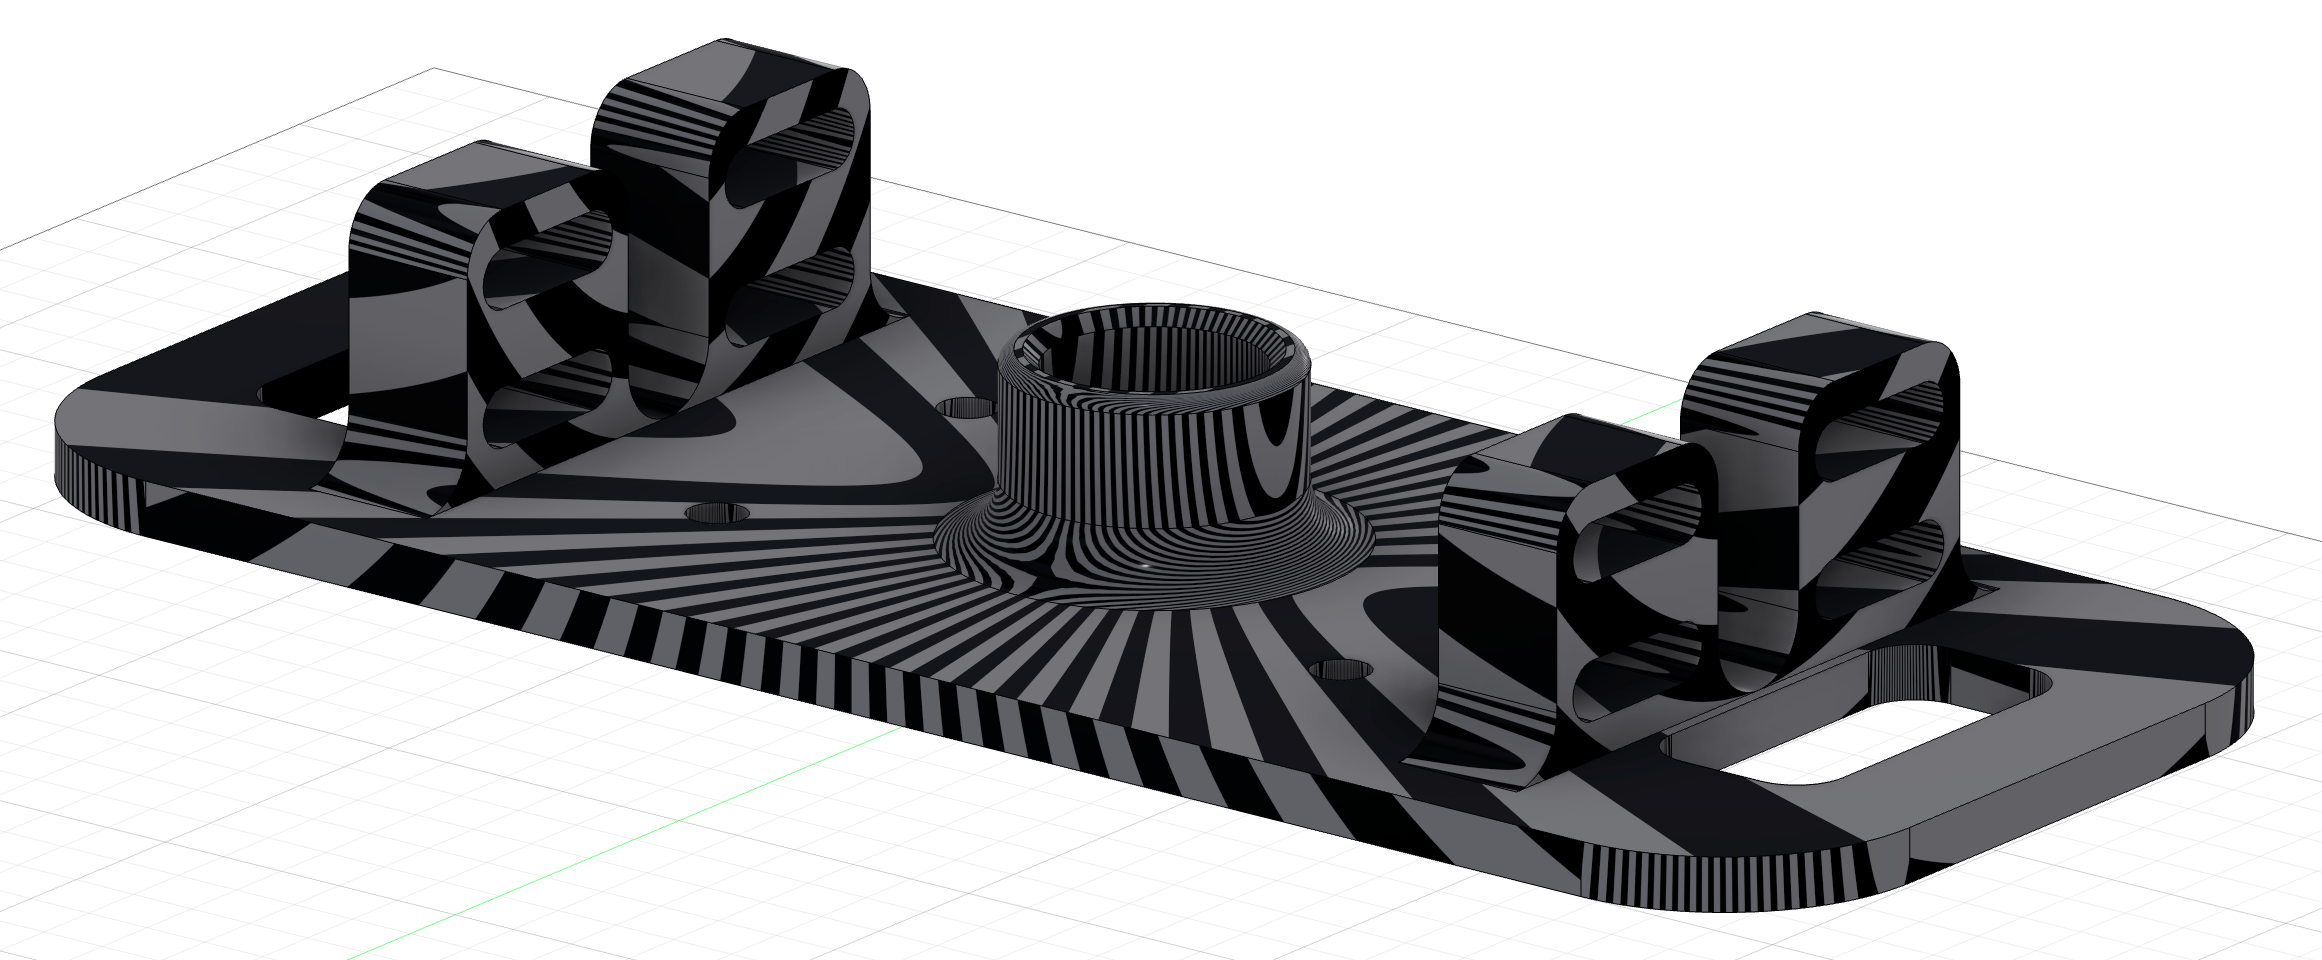
\includegraphics[width=\textwidth]{images/ZEBRA/baseMotorSupport.png}
    \caption{ZEBRA analysis of the base motor support}
    \label{fig:zebra_base_motor_support}
\end{figure}

\begin{figure}[H]
    \centering
    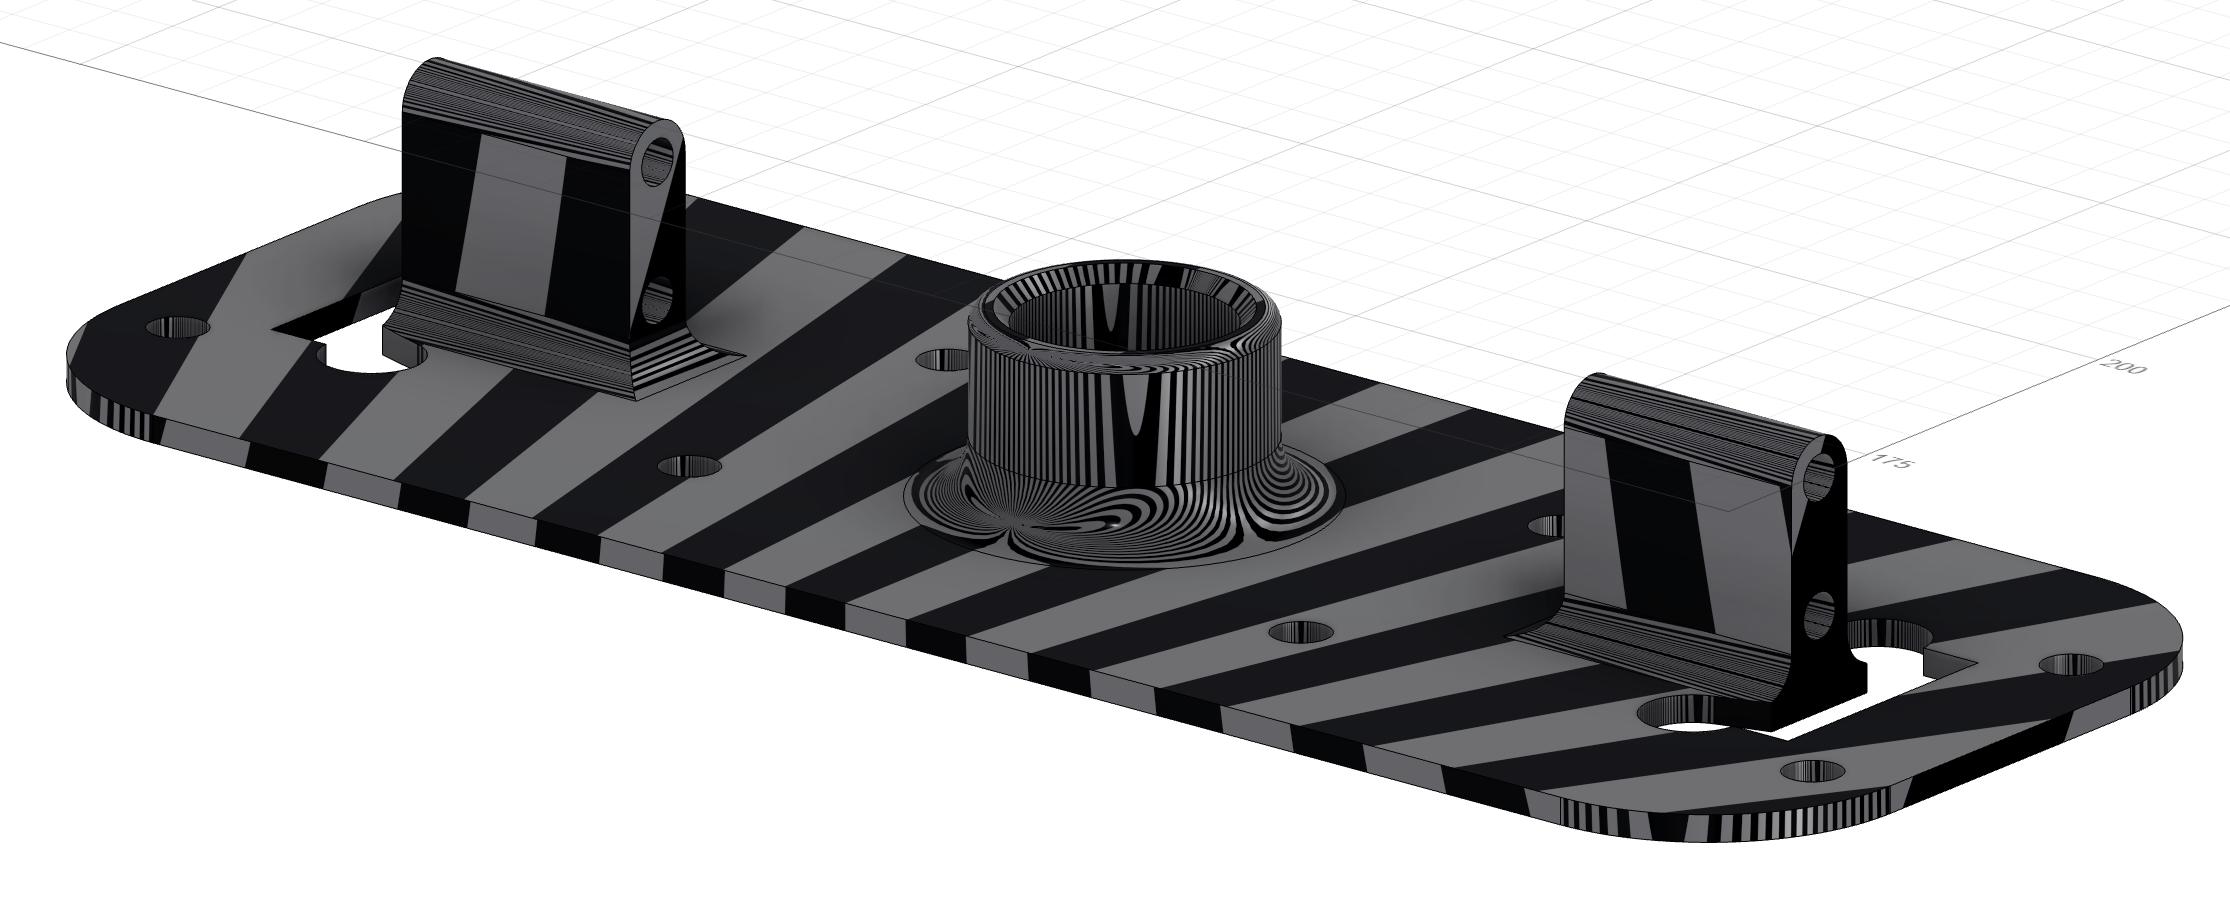
\includegraphics[width=\textwidth]{images/ZEBRA/basePlatform.png}
    \caption{ZEBRA analysis of the base platform}
    \label{fig:zebra_base_platform}
\end{figure}

   
\newpage

\section{Conclusion and Future Work}
\subsection{Summary of Findings}
This thesis presented the design and analysis of a low-cost suspension system tailored for a heavy-duty AMR. The proposed solution effectively addresses the primary challenges posed obstacles on regular industrial surfaces, and varying payload distributions, ensuring consistent and reliable performances. The work focused on developing a robust, spring-based passive suspension system capable of absorbing shocks and maintaining stability without relying on complex or expensive active control mechanisms.

Key findings of this research include the successful implementation and validation of the suspension design through both analytical calculations and experimental testing. Static and fatigue analyses confirmed that the system satisfies the required safety factors, offering sufficient durability and mechanical reliability under standard operating conditions. Additionally, 
FEM simulations further validated the design by accurately predicting stress concentrations and deformation behaviors, demonstrating that the structure can withstand payloads without risk of failure.

Despite the positive outcomes, the study also identified some limitations of the proposed design. The primary drawback lies in the absence of active control, which reduces the system's responsiveness to rapidly changing dynamic environments or uneven terrain. Moreover, the torque generated by the payload asymmetry introduces additional stress on the suspension components which could lead to premature failure, if not properly accounted.

\subsection{Outlook and Recommendations}
Future work should focus on further optimizing the suspension system to address its current limitations and unlock additional performance improvements. One promising direction involves the integration of active damping mechanisms or adaptive control strategies, which could significantly enhance the responsiveness to real-time changes in terrain and payload.

In addition to control enhancements, future research should investigate the use of advanced materials that could improve mechanical features. By incorporating lightweight yet durable materials such as carbon fiber, reinforced polymers or high-performance thermoplastics, it may be possible to reduce the overall mass of the suspension without compromising its structural integrity.

Lastly, future development could benefit from the integration of real-time data acquisition systems within the suspension structure. Embedding sensors to monitor load, vibration, and wear over time would allow for predictive maintenance strategies and provide valuable insights into long-term performance, turning the system into a more intelligent suspension systems.

\newpage
\printbibliography
\end{document}